\documentclass{tran-l}
%\usepackage{natbib}
\usepackage[square,sort,comma,numbers]{natbib}
\usepackage[T1]{fontenc}
\usepackage[utf8]{inputenc}
%\usepackage[icelandic]{babel}
\setcitestyle{square}
\usepackage{amsmath,amssymb,amsfonts,amsthm}
\usepackage{mathtools}
\usepackage{mathrsfs}
\usepackage{chemfig}
\usepackage{chemformula}
\usepackage{centernot}
\usepackage{booktabs}
\usepackage{enumitem}  
\usepackage{url}
\usepackage{xcolor}
\definecolor{navy}{RGB}{0,0,128}
\definecolor{royalblue}{RGB}{65,105,225}
\usepackage{hyperref}
\hypersetup{
    linktocpage,
    colorlinks,
    citecolor=royalblue,
    filecolor=black,
    linkcolor=royalblue,
    urlcolor=black
}
\usepackage[left=3cm, right=3cm]{geometry}
\usepackage{braket}
\usepackage{physics}
\usepackage{amscd}
\usepackage{tikz-cd} 
%\usepackage{tikz}
\usepackage{tikz-3dplot}


\usepackage{algorithm}
\usepackage{algpseudocode}
\usetikzlibrary{arrows.meta,positioning,shapes.geometric,fit,backgrounds,calc}
\usepackage{adjustbox}
\definecolor{accent}{RGB}{0,100,148} % deep teal; change if desired
\usetikzlibrary{shapes.arrows}
\usetikzlibrary{positioning}
\usepackage{calc}
\usepackage{float}
\tikzset{%
  symbol/.style={
    draw=none,
    every to/.append style={
      edge node={node [sloped, allow upside down, auto=false]{$#1$}}
    },
  },
}

%\usetikzlibrary{positioning}
%\usetikzlibrary{arrows}
\usetikzlibrary{decorations.pathmorphing}


\let\LATEXth\th
\let\gbth\th
\let\th\LATEXth


\usepackage{caption}
\captionsetup{justification   = raggedright,
              singlelinecheck = false}
%     Update the information and uncomment if AMS is not the copyright
%     holder.
%\copyrightinfo{2009}{American Mathematical Society}

\newtheorem{theorem}{Theorem}[section]
\newtheorem{lemma}[theorem]{Lemma}

\newtheorem{question}{Question}
\newtheorem{proposition}[theorem]{Proposition}
\newtheorem{corollary}[theorem]{Corollary}
\newtheorem*{summary*}{Summary}
\newtheorem{conjecture}{Conjecture}

\theoremstyle{definition}
\newtheorem{definition}[theorem]{Definition}
\newtheorem{example}[theorem]{Example}
%\newtheorem*{"definition"}{"Definition"}
\newtheorem{xca}{Exercise}



\theoremstyle{remark}
\newtheorem{remark}[theorem]{Remark}

\numberwithin{equation}{section}

\DeclareMathOperator{\Vol}{Vol}
\DeclareMathOperator{\vol}{Vol}
\DeclareMathOperator{\Hol}{Hol} 
\DeclareMathOperator{\DD}{DD} 
\DeclareMathOperator{\End}{End} 
%\DeclareMathOperator{\Hom}{Hom} 
%\DeclareMathOperator{\im}{im}
\DeclareMathOperator{\Ker}{Ker}
\DeclareMathOperator{\Imop}{Im}
\DeclareMathOperator{\Coker}{Coker}
\DeclareMathOperator{\Hom}{Hom}
%\DeclareMathOperator{\End}{End}
\newcommand{\Cech}{Čech}
\usepackage{amsmath,amssymb}
%\newcommand{\F}{\mathcal{F}}
\newcommand{\M}{\mathcal{M}}
\newcommand{\A}{\mathcal{A}}
\newcommand{\D}{\mathbf{D}}
\newcommand{\Open}{\mathbf{Open}}
\newcommand{\Cat}{\mathbf{Cat}}
\newcommand{\Dens}{\mathbf{Dens}}
\newcommand{\CPM}{\mathbf{CPM}}
\newcommand{\FHilb}{\mathbf{FHilb}}
\newcommand{\QChan}{\mathbf{QChan}}
\newcommand{\K}{\mathcal{K}}
\newcommand{\R}{\mathcal{R}}
\newcommand{\G}{\mathcal{G}}
\newcommand{\checkc}{\check c}
\newcommand{\diamondnorm}[1]{\lVert#1\rVert_{\diamond}}



\newcommand{\cN}{\mathcal{N}}
\newcommand{\Z}{\mathbb{Z}}
\newcommand{\SU}{\mathrm{SU}}
\newcommand{\U}{\mathrm{U}}
\newcommand{\TMF}{\mathrm{TMF}}
\newcommand{\SQFT}{\mathrm{SQFT}}
\newcommand{\vectpsi}{\vec{\psi}}
\newcommand{\Herm}{\mathrm{Herm}}
\newcommand{\id}{\mathrm{id}}
\newcommand{\Sep}{\mathrm{Sep}}
\newcommand{\cone}{\mathrm{cone}}
\newcommand{\Ad}{\mathrm{Ad}}
\newcommand{\Ind}{\mathrm{Ind}}
\newcommand{\ind}{\mathrm{ind}}
%\newcommand{\ch}{\mathrm{ch}}
\newcommand{\im}{\mathrm{im}}
%\newcommand{\Hol}{\mathrm{Hol}}
\newcommand{\sgn}{\mathrm{sgn}}
\newcommand{\ad}{\mathrm{ad}}

%\section{Notation\,/\,Macros}
%\newcommand{\mathcal{H}}[1]{\mathcal H(#1)}           % Hermitian linear envelope
\newcommand{\sep}{\mathsf{sep}}  
%\newcommand{\Sep}{\mathsf{Sep}}       
\newcommand{\F}[1]{\mathcal F(#1)}           
\newcommand{\Ck}[1]{C^{#1}}                 
\newcommand{\dC}[1]{\delta^{#1}}         


\usepackage[utf8]{inputenc}
\usepackage{bxcjkjatype}
\newcommand{\wye}{\mbox{\begin{uCJK}\UTF{3091}\end{uCJK}}} %ゑ
\newcommand{\wyi}{\mbox{\begin{uCJK}\UTF{3090}\end{uCJK}}} %ゐ
\newcommand{\nn}{\mbox{\begin{uCJK}\UTF{3093}\end{uCJK}}} %ん
\newcommand{\ru}{\mbox{\begin{uCJK}\UTF{308B}\end{uCJK}}} %る
\newcommand{\no}{\mbox{\begin{uCJK}\UTF{306E}\end{uCJK}}} %の
\newcommand{\se}{\mbox{\begin{uCJK}\UTF{305B}\end{uCJK}}} %せ
\newcommand{\so}{\mbox{\begin{uCJK}\UTF{305D}\end{uCJK}}} %そ
\usepackage{multirow} 

\newcommand{\ki}[1]{{\color[rgb]{0,0,1}{[K.I.: #1]}}}
\definecolor{QGLBlue}{RGB}{65,105,225}   % RoyalBlue-ish
\definecolor{QGLRed}{RGB}{203,65,84}     % BrickRed-ish
\definecolor{QGLGreen}{RGB}{34,139,34}   % ForestGreen-ish

\newcommand{\hlEq}[1]{%
  \begingroup\setlength{\fboxsep}{2pt}%
  \colorbox{QGLBlue!5}{$\displaystyle #1$}%
  \endgroup}

\newcommand{\hlLine}[1]{%
  \begingroup\setlength{\fboxsep}{1.5pt}%
  \colorbox{QGLRed!12}{\textbf{#1}}%
  \endgroup}

\newcommand{\hlDef}[1]{%
  \begingroup\setlength{\fboxsep}{1pt}%
  \colorbox{QGLGreen!15}{\textbf{#1}}%
  \endgroup}

\definecolor{QGLItem}{RGB}{255,245,204} % soft fill color

\usepackage[most]{tcolorbox}
\definecolor{QGLItem}{RGB}{65,105,225}
\newtcolorbox{HLblock}{enhanced,breakable,
  colback=QGLBlue!5, colframe=QGLBlue!5, % same color, no visible frame
  boxrule=0pt, arc=0pt, outer arc=0pt,
  left=2pt,right=2pt,top=1.5pt,bottom=1.4pt}

\begin{document}

\title{Quantum Entanglement as a Cohomological Obstruction}

\author{Kazuki Ikeda}
\address{}
\curraddr{}

\email{kazuki.ikeda@umb.edu}
\address{Department of Physics, University of Massachusetts Boston, USA}
\address{Center For Nuclear Theory, Department of Physics and Astronomy, Stony Brook University, USA}

\thanks{The author expresses gratitude to Steven Rayan for his careful reading of the manuscript and for his invaluable comments. The author is also grateful to Myungbo Shim for useful discussions. This work was partially supported by the NSF under Grant No. OSI-2328774.}

%\subjclass is required.
%\subjclass[2010]{Primary}
\subjclass[2020]{81P40 (Primary),%quantum theory 
14D24, %Geometric Langlands program
14F05, %Vector bundles, sheaves, related constructions.
58J20, %Index theory 
53C05 %Sheaf cohomology
}
\date{}

\dedicatory{}
%    Abstract is required.
\begin{abstract}
We recast quantum entanglement as a cohomological obstruction to reconstructing a global quantum state from locally compatible information. We address this by considering presheaf cohomologies of states and entanglement witnesses. Sheafification erases the global-from-local signature while leaving within-patch multipartite structure, captured by local entanglement groups introduced here. For smooth parameter families, the obstruction admits a differential-geometric representative obtained by pairing an appropriate witness field with the curvature of a natural unitary connection on the associated bundle of amplitudes. We also introduce a \emph{Quantum Entanglement Index} (QEI) as an index-theoretic invariant of entangled states and explain its behavior. Finally, we outline a theoretical physics approach to probe these ideas in quantum many-body systems and suggest a possible entanglement-induced correction as an experimental target.
\end{abstract}
\maketitle
\tableofcontents
%\newpage
\section{Introduction}
\noindent
\textbf{Preliminaries.}
Quantum entanglement is the organizing principle of quantum systems, representing the defining nonclassical correlation in quantum systems, that facilitates quantum information capabilities and structures the landscape of quantum phases. By definition, an entangled state shares information across the whole system through nonclassical correlations. This indicates that local information obtained by tracing out subsystems need not determine the global state. Motivated by this thought, we test entanglement through a reconstruction question: when do locally compatible marginals assemble into a global state, and when is such a state unique? In algebro-geometric terms, the presheaf of states may fail to satisfy the sheaf axioms in the presence of entanglement: gluing can fail, and even when gluing is possible, uniqueness can fail. In this setting, entanglement appears as a cohomological obstruction to global reconstruction. Reduced density operators may agree on all overlaps while a global state is not unique.

A variety of quantitative measures of entanglement have been introduced, ranging from entanglement entropy for pure states, to entanglement of formation, distillable entanglement, and relative entropy of entanglement for mixed states, to more computationally motivated quantities such as concurrence and negativity (see, e.g., \cite{Horodecki:1996nc,2001quant.ph..1032T,Guhne:2008qic,umegaki1962conditional}). These are real‑valued functions of states and are useful for analysis and numerics, but they are not directly accessible experimentally. By contrast, we work with entanglement witnesses, which are Hermitian observables. As physical observables, their expectation values provide testable certificates for separability or inseparability. We also use their global organization to examine compatibility across patches.

The aim of this work is to develop an algebro-geometric and topological framework in which entanglement is expressed as a cohomological obstruction to gluing local data. We proceed in two parts. On the discrete side, we organize states and entanglement witnesses into presheaves and express obstructions as Čech cohomology classes. On the geometric side, for smooth parameter families of states we obtain a Chern–Weil representative by pairing a parallel family of witnesses with the curvature of a natural unitary connection on the associated bundle of amplitudes (see \cite{UHLMANN1986229,Petz:1999xrh,BottTu}). This links the reconstruction problem to standard objects in differential geometry. The result is a correspondence between compatibility data and characteristic classes on parameter space, developed in a finite‑dimensional setting and suggesting broader interactions with geometry.

\vskip0.3cm
\noindent
\textbf{The gluing problem.}
Fix a finite index set $I=\{1,\dots,N\}$ and finite dimensional complex Hilbert spaces $H_j\simeq\mathbb C^{d_j}$. For every nonempty $U\subseteq I$, put
\[
H_U:=\bigotimes_{j\in U}H_j,\qquad
\mathcal D(U):=\{\rho\in\mathrm{End}(H_U)\mid \rho=\rho^\dagger,\ \rho\ge0,\ \mathrm{Tr}\,\rho=1\}.
\]
Let $\mathcal S\subset \mathcal D$ be any restriction-stable presheaf of quantum states: for each $U\subseteq I$, $\mathcal S(U)\subseteq\mathcal D(U)$ and for all $V\subseteq U$ one has $\mathrm{Tr}_{U\setminus V}\,\mathcal S(U)\subseteq\mathcal S(V)$ (partial trace on the discarded factor is a common choice for a restriction map). With restriction maps $r^U_{V}:S(U)\to S(V)$ for $V\subset U$, define the $0$-cochains by $C^0(\mathcal U,S):=\prod_{i} S(U_i)$ and the $1$-cochains $C^1(\mathcal U,S):=\prod_{i<j} S(U_{ij})$ with $U_{ij}:=U_i\cap U_j$. Let $H^0$ be the equalizer of the two families of restriction maps:
\[
H^0(\mathcal U,S)
:=\Big\{(s_i)_i\in\textstyle\prod_i S(U_i)\ :\ r^{U_i}_{U_{ij}}(s_i)=r^{U_j}_{U_{ij}}(s_j)\ \text{ for all }i<j\Big\}.
\]

When each $S(U)$ is an abelian group and the restrictions are homomorphisms, $\delta^0:C^0(\mathcal U,S)\to C^1(\mathcal U,S)$ is
\[
(\delta^0 s)_{ij}\;:=\; r^{U_i}_{U_{ij}}(s_i)\;-\; r^{U_j}_{U_{ij}}(s_j)\qquad (i<j),
\]
and
\[
H^0(\mathcal U,S)=\ker\delta^0.
\]


\begin{example}
Let $\mathcal V(U)=\mathrm{Herm}(H_U)$ equipped with the trace pairing $\langle X,Y\rangle = \mathrm{Tr}(XY)$. We consider the usual restriction given by partial trace. Writing $X=(X_i)_i\in\prod_i \mathcal V(U_i)$, for each overlap $U_{ij}$ we have
\[
(\delta^0 X)_{ij}
\;=\;
\Tr_{\,U_i\setminus U_{ij}}(X_i)\;-\;\Tr_{\,U_j\setminus U_{ij}}(X_j)
\;\in\; V(U_{ij}).
\]
Thus
\[
H^0(\mathcal U,\mathcal V)
=\Big\{(X_i)_i:\ \Tr_{\,U_i\setminus U_{ij}}(X_i)=\Tr_{\,U_j\setminus U_{ij}}(X_j)\ \text{for all }i<j\Big\}.
\]
\end{example}

\vskip0.3cm
The map
\[
j_{\mathcal U}:\ \mathcal S(I)\longrightarrow H^0(\mathcal U,\mathcal S),\qquad
\rho\longmapsto \bigl(\rho|_{U_i}\bigr)_i
\]
encodes the sheaf axiom on $(\mathcal U,\mathcal S)$. Its failure appears in two distinct modes:
\begin{HLblock}
\begin{enumerate}[label=\textbf{(\Alph*)},leftmargin=*]
\item\label{A}\textbf{Gluing failure:} $j_{\mathcal U}$ is not surjective. There exist compatible marginals
$\{\rho_i\in\mathcal S(U_i)\}_i$ (i.e. agreeing on all overlaps) which admit no global $\rho\in\mathcal S(I)$
with $\mathrm{Tr}_{I\setminus U_i}\rho=\rho_i$ for every $i$.
\item\label{B}\textbf{Non-uniqueness:} $j_{\mathcal U}$ is not injective. There exist two distinct global states
$\rho_1\neq\rho_2\in\mathcal S(I)$ with identical marginals on every $U_i$.
\end{enumerate}
\end{HLblock}
Whether \ref{A} or \ref{B} occurs depends on the choice of $\mathcal S$. When $\mathcal S$ is a sheaf, both pathologies are absent by definition. In physically relevant presheaves, however, entanglement forces one (or both) to appear. For instance, for $\mathcal S=\mathcal D$ and $I=\{1,2\}$ the four Bell states $\ket{\Psi^\pm}=\frac{\ket{01}\pm\ket{10}}{\sqrt{2}},\ket{\Phi^\pm}=\frac{\ket{00}\pm\ket{11}}{\sqrt{2}}$ share the same single–site marginals (\(\Tr_{\{i\}}\ket{\Psi^\pm}\bra{\Psi^\pm}=\Tr_{\{i\}}\ket{\Phi^\pm}\bra{\Phi^\pm}=\frac{\mathbf 1}{2},~i\in\ I\)), so the restriction $\mathcal D(I)\to\mathcal D(\{1\})\times\mathcal D(\{2\})$ is not injective. This is an instance of \ref{B}. For the broader theme of uniqueness of state extensions, see \cite{25f8c26d-c81c-39c1-9128-a71146ac84ff,33675660-3119-37a8-a5d2-fa5a40dfb227,7f2d66a9-2d0a-3ab6-8756-1cda100696a6}. 

An immediate example for \ref{A} is when $\mathcal{S}$ is a presheaf of pure states. For the pure-state presheaf $\mathcal P\subset\mathcal D$, nontrivial pure patches typically obstruct gluing: a global pure extension exists if and only if each local pure state is product on their patch, otherwise no global pure extension exists. This statement can be summarized as follows:
\begin{proposition}\label{prop:pure-fail}
Let $\mathcal U=\{U_i\}_{i=1}^m$ be a partition of $I$. Given pure local states $\rho_i=|\psi_i\rangle\!\langle\psi_i|\in P(U_i)$, there exists a unique global pure state $\rho=|\Psi\rangle\!\langle\Psi|\in P(I)$ with $\rho|_{U_i}=\rho_i$ for all $i$, namely $|\Psi\rangle=\bigotimes_{i=1}^m |\psi_i\rangle$. Conversely, for a global pure state $\rho=|\Psi\rangle\!\langle\Psi|$ the following are equivalent: (i) $\rho|_{U_i}$ is pure for every $i$; (ii) $|\Psi\rangle=\bigotimes_{i=1}^m |\psi_i\rangle$ (a product across the partition).
\end{proposition}


Our approach is entirely in the density-matrix (operator) formalism: we pose gluing as a problem for a presheaf of state spaces and measure its failures by cohomological obstructions \(R^0\) (Definition \ref{def:compat-defect}) for non–uniqueness \ref{B} and the local entanglement groups \(E^q\) (Definition \ref{def:Eq-ordered-cosimplicial}) for within-patch multipartite content \ref{A} with operational (separable-witness) certificates. This complements the spectral/representation theoretic marginal program, where necessary constraints on compatible spectra are obtained via moment map \cite{guillemin1982convexity,kirwan1984convexity,berenstein2000coadjoint} and via marginal spectra analyses \cite{Christandl2006,2014CMaPh.332....1C}. For a math treatment linking quantum marginals to projections of coadjoint/orbital measures, see Collins–McSwiggen \cite{Collins:2021xyq}. Our approach is orthogonal to these methods. Conceptually, our use of presheaves echoes the sheaf-theoretic account of contextuality/nonlocality as obstructions to global sections \cite{abramsky2011sheaf}, though here the presheaf consists of density operators. More specifically, our obstruction $R^0$ measures the degree of non-uniqueness, while the invariants $E^q$ capture the local entanglement that either prevents or allows gluing. Through the witness characterization, these quantities are equivalent to determining whether certain pairings with separable witnesses vanish or not. This is discussed from the perspective of quantum information theory. The use of entanglement witnesses as separating functionals for the cone of separable states goes back to the Horodecki criterion \cite{Horodecki:1996nc}, with systematic expositions by Terhal \cite{2001quant.ph..1032T} and G{\"u}hne–T{\'o}th \cite{Guhne:2008qic}.


\vskip0.3cm
\noindent
\textbf{Witness presheaf and obstructions.}
We encode entanglement by witnesses. For $U\subseteq I$ let the witness cone be
\begin{equation}\label{eq:Witt}
   \mathsf{Wit}(U)
   :=\bigl\{W=W^\dagger\in\End(H_U)\ \big|\ 
       \Tr(W\sigma)\ge0\ \ \forall\,\sigma\in\Sep(U)\bigr\},
\end{equation}
and put $\mathcal W(U):=\mathrm{span}_{\mathbb R}\mathrm{Wit}(U)$. Here \(\Sep(U)\) is the set of all separable states on $U$. For an inclusion \(V\subseteq U\) define the restriction
\begin{equation}\label{eq:w-restr}
   r^U_{V}:\mathcal W(U)\to\mathcal W(V),\qquad
   r^U_{V}(W):=\Tr_{U\setminus V}\!\bigl[W\,(\mathbf 1_V\otimes\tau_{U\setminus V})\bigr],
\end{equation}
with a fully separable state \(\tau\) on the traced factor. We fix, once and for all, a sitewise faithful state $\{\tau_j\}_{j\in I}$ and set $\tau_S := \bigotimes_{j\in S}\tau_j$ for every $S\subset I$. With this multiplicative rule, we see that the witness restriction
$r^{U}_{V}(W):=\Tr_{U\setminus V}\!\big[\,W\,(\mathbf{1}_V\otimes \tau_{U\setminus V})\big]$
satisfies the axiom: for $U_3\subset U_2\subset U_1$,
\[
r^{U_2}_{U_3}\circ r^{U_1}_{U_2} \;=\; r^{U_1}_{U_3}.
\]
Indeed, functoriality follows from $\tau_{U_1\setminus U_3}=\tau_{U_2\setminus U_3}\otimes \tau_{U_1\setminus U_2}$ and the cyclicity of the trace. This fixed choice will be used throughout.


We use $W$ as functionals on $\mathcal V(U):=\mathrm{Herm}(H_U)$ via the trace pairing. In finite dimension, one has $\mathcal{W}(U)=\mathcal V(U)$ (Proposition~\ref{prop:wit-separate-span}), and the linear Čech complex contracts in positive degrees by product state extensions (Proposition~\ref{prop:degree0}). Consequently, $H^{>0}(\mathcal U, \mathcal{W})=0$ for every finite cover $\mathcal U$, and there is no nontrivial group-valued ``existence obstruction'' at degree~1. Existence of a global state is instead a cone-feasibility question certified by duality: the certificates for positive semi-definite (PSD) and separable infeasibility are given in Propositions~\ref{prop:state-level-extension} and~\ref{prop:farkas}, which are extensions of Farkas's lemma. Uniqueness is measured by the kernel $R^0=\ker j$ of the degree–0 map. Operationally, vanishing of a Čech class built from local states is equivalent to pairing to zero against every compatible family in \(C^\bullet(\mathcal U,\mathcal W)\) (Theorem~\ref{thm:witness-vanish}).



For each region $U$ we view $\mathcal S(U)\subset\mathcal D(U)$ as a presheaf of states with restriction by partial trace $r^U_V:\mathcal S(U)\to\mathcal S(V)$ for $V\subset U$. The corresponding witness assignment (Definition \ref{def:dualcone})
\[
\mathcal W(U):=C^*_{\mathrm{sep}}(U)
\]
pulls back along inclusions by the adjoints $r^{U}_V{}^{\!\dagger}$ so that the trace pairing is natural: $\langle r^{U}_V{}^{\!\dagger}W,\,X\rangle=\langle W,\,r^U_V X\rangle$. On a cover, entanglement appears as nonzero entanglement obstruction classes for the operator presheaf. Compatible witness cochains certify nonvanishing by producing strictly negative total pairings. Within a single patch, the ancilla column built from state insertion and single‑slot resets has cohomology $E^q(U)$ that records local multipartite depth. A class is nonzero exactly when some separable witness on $U^{(q+1)}$ yields a negative signed‑reset pairing. For smooth parameter families, a parallel witness field pairs with the state Čech class and produces the de~Rham class $\big[(2\pi i)^{-k}\mathrm{Tr}(WF^{k})\big]$ (Theorem~\ref{thm:global-uhl}). In this way the presheaf of witnesses acts as a dual detector for the presheaf of states.


\vskip0.3cm
\noindent
\textbf{Sheafification.}
Sheafification of a presheaf $\mathcal S$ produces a sheaf $\mathcal S^\#$ and a natural map $\eta:\mathcal S\to\mathcal S^\#$ with the property that, on any fixed cover $\mathcal U=\{U_i\}$, the degree-$0$ restriction $j^\#_{\mathcal U}:\mathcal S^\#(U)\!\xrightarrow{\;\sim\;} H^0(\mathcal U,\mathcal S^\#)$ is bijective. Thus all gluing and separatedness issues visible on $\mathcal U$ are removed, and any two global states that are indistinguishable by all restrictions to $\mathcal U$ (and its refinements) become equal in $\mathcal S^\#$. However, this does not mean that the underlying state is separable: sheafification erases only the ``global vs.\ local'' signature of entanglement. Patchwise multipartite structure (as measured, e.g., by the local entanglement groups $E^q$ (Definition \ref{def:Eq-ordered-cosimplicial}) attached to a single patch) may still be present, but it is invisible to the local tests. Therefore $\overline{E}^q=\varinjlim_{\mathcal U} E^q(\mathcal U)$ can remain non‑zero after sheafification (Theorem \ref{thm:completeness-weak}). In particular, every computation that depends solely on local projections and their linear combinations (e.g.\ $\sum_i \Tr[W_i\,\rho|_{U_i}]$) factors through $\eta$ and is therefore preserved under sheafification on that cover.

A presheaf on a finite cover behaves as a distributed data structure: each $U_i$ stores a local record. Sheafification performs a natural consistency completion and a quotient by observational equivalence. Here any two records that produce the same observable outcomes under projections are considered equivalent. After sheafification, the remaining invariants live in the classical side. By contrast, non-classical features we study here reside in the presheaf picture prior to sheafification.


\vskip0.3cm
\noindent
\textbf{Quantum Entanglement Index.}
Section~\ref{sec:obstruction} organize states and witnesses into a presheaf and express ``global-from-local'' failures as Čech classes. When the local data vary smoothly over a parameter manifold $X$, the obstruction acquires a differential geometric description. Section~\ref{sec:diff-form-obstruction} then explore these obstructions from the perspective of differential geometry on parameter space: given a smooth family of full‑rank states \(\rho:X\to\mathcal D_{\mathrm{full}}(H)\), we pass to the pullback amplitude bundle
\[
E_\rho:=\{(x,W)\in X\times GL(H): WW^\dagger=\rho(x)\}\to X,
\]
which is a principal \(U(r)\)–bundle.  In this setting the Čech cocycle built from local amplitudes and their unitary transitions is compared with de~Rham cohomology: for a smooth $A$–parallel witness field $W$, the ordered pairing equals the Chern–Weil form (Theorem \ref{thm:global-uhl}):
\[
\big\langle W,\ [\delta^k(u)]_{\check C}\big\rangle
\;=\;
\Big[\,(2\pi i)^{-k}\,\Tr\big(WF_A^{\,k}\big)\,\Big]_{\!dR},
\]
so the obstruction class is represented on $X$ by the closed forms $(2\pi i)^{-k}\Tr(WF_A^{k})$. Physically, it can be understood as an extension of Berry/TKNN number (see Section \ref{sec:phys}). 


This geometric counterpart converts witness‑certified obstructions into characteristic classes on $X$ and furnishes the input for the index‑theoretic refinement that follows in Section~\ref{sec:QGL}. Let $(E,A)$ be a Hermitian bundle with unitary connection and let $W\in\Gamma(\mathrm{End}(E))$ be an $A$–parallel witness field on $X$. Writing $S:=\mathrm{sgn}(W)$ and $F_A$ for the curvature, the \emph{Quantum Entanglement Index} (QEI) (Definition~\ref{def:quantum-index}) records the difference of Dirac indices seen by the $S$–positive/negative sectors:
\[
\mathrm{Ind}_S\big(D_X\!\otimes E\big)
:= \mathrm{ind}\big(D_X\!\otimes E_+\big) - \mathrm{ind}\big(D_X\!\otimes E_-\big)
= \Big\langle \widehat A(TX)\wedge \mathrm{Tr}\big(Se^{F_A/2\pi i}\big),[X]\Big\rangle .
\]
Thus an $A$–parallel witness grades the theory by an integer, and this grading is topological on parameter space:
\begin{figure}[H]
\centering
\begin{tikzcd}[column sep=huge]
\mathsf{QGL}(X):=\{(E,A,W):D_AW=0\}
\arrow[r, dashed]
& \mathcal{D}\mathrm{-mod}(\mathrm{Bun}_G)
\end{tikzcd}
\end{figure}

\noindent
We use this index to grade automorphic data: to a spectral datum $(E,A,W)$ we associate an automorphic object together with its $\mathbb Z$–degree $\mathrm{Ind}_S$. In this way, the quantum entanglement refinement overlays the classical automorphic category with a natural grading determined by the witness. A Hecke functor then has a quantized effect on the grading. If $H_{x,\lambda}$ is a Hecke modification of coweight $\lambda$ at $x$, its action shifts the QEI by the signed charge $\langle S,\lambda\rangle$:
\[
\mathrm{Ind}_S\!\left(H_{x,\lambda}\,\mathsf{Aut}_{(E,W)}\right)
=\mathrm{Ind}_S\!\left(\mathsf{Aut}_{(E,W)}\right)+\langle S,\lambda\rangle .
\]
The correspondence can be summarized in the following diagram:
\begin{figure}[H]
\centering
\begin{tikzcd}[column sep=large]
& \mathrm{Hecke}_x \arrow[dl,"p_1"'] \arrow[dr,"p_2"] & \\
\mathsf{Aut}_{(E,W)} \arrow[rr, dashed, "H_{x,\lambda}"] \arrow[d, "\mathrm{Ind}_S" left] 
&& \mathsf{Aut}_{(E,W)} \arrow[d, "\mathrm{Ind}_S"] \\
\mathbb Z \arrow[rr, "{+\langle S,\lambda\rangle}"] && \mathbb Z
\end{tikzcd}
\end{figure}
\noindent
This expresses that Hecke modifications induce discrete jumps between entanglement sectors, which can be interpreted as an entanglement-induced quantum phase transition in quantum many-body systems. The automorphic object is transformed while its degree is shifted by $\langle S,\lambda\rangle$. The index also admits a differential–geometric realization.

\vskip0.3cm
\noindent
\textbf{Bridging to geometric Langlands.}
We begin with fundamental structures of the geometric Langlands correspondence. It is expected that flat ${}^{L}\!G$–local systems on $X$ correspond to $\mathcal{D}$–modules on $\mathrm{Bun}_G$:
\begin{figure}[H]
\centering
\begin{tikzcd}[column sep=large]
\mathrm{Loc}_{\,^{L}\!G}(X) \arrow[r, dashed, "\mathrm{GL}"] 
& \mathcal{D}\mathrm{-mod}(\mathrm{Bun}_G)
\end{tikzcd}
\end{figure}
\noindent
Then the Hecke correspondence at a point $x\in X$ gives endofunctors of the automorphic category by convolution with spherical kernels. 
Concretely, for every $V\in\mathrm{Rep}({}^{L}\!G)$ one has the functor
\[
H_{x,V}\;=\;p_{2!}\!\left(p_1^{*}(-)\otimes\mathcal S_{V}\right),
\]
assembled from the correspondence:
\begin{figure}[H]
\centering
\begin{tikzcd}
& \mathrm{Hecke}_x \arrow[dl,"p_1"'] \arrow[dr,"p_2"] & \\
\mathrm{Bun}_G \arrow[rr, dashed,
"{H_{x,V}=\,p_{2!}\big(p_1^{*}(-)\otimes\mathcal S_{V}\big)}"'] 
&& \mathrm{Bun}_G
\end{tikzcd}
\end{figure}

\noindent
For a local system $E$, the associated automorphic object $\mathrm{Aut}_E$ is a Hecke eigensheaf: for every $x\in X$ and $V\in\mathrm{Rep}({}^{L}\!G)$,
\[
H_{x,V}(\mathrm{Aut}_E)\;\simeq\;(V_{E_x})\otimes \mathrm{Aut}_E,
\]
so the fiber $V_{E_x}$ plays the role of the eigenvalue on the automorphic side.

\bigskip
\noindent
Finally, the spherical geometric Satake equivalence identifies the geometric inputs for the kernels: $G(\mathcal O)$–equivariant (perverse) sheaves (or $\mathcal{D}$–modules) on the affine Grassmannian are equivalent to $\mathrm{Rep}({}^{L}\!G)$. Under this identification, the kernel $\mathcal S_V$ corresponds to the representation $V$.
\begin{figure}[H]
\centering
\begin{tikzcd}[column sep=huge]
\mathsf{Perv}_{G(\mathcal O)}(\mathrm{Gr}_G) 
\arrow[r, "\mathrm{Satake}", "\simeq"'] 
& \mathrm{Rep}\!\left(^{L}\!G\right)
\end{tikzcd}
\end{figure}

\noindent
In our quantum refinement (Section~\ref{sec:QGL}), the same Hecke functors would act on automorphic data equipped with the integral grading given by the QEI, and Hecke modifications of coweight~$\lambda$ shift the degree by $\langle S,\lambda\rangle$. While the traditional framework remains intact, our approach here introduces a natural integer grading on the automorphic side that is sensitive to the entanglement response.


\section{\label{sec:obstruction}Quantum entanglement from the viewpoint of topology}
\subsection{\label{sec:presheaf}Presheaf of quantum states}
For each finite subsystem $U \subseteq I$, let
\[
   \mathcal V(U) := \mathrm{Herm}(H_U)
\]
be the real vector space of Hermitian operators on $H_U$, equipped with the trace pairing $\langle X,Y\rangle = \mathrm{Tr}(XY)$.

\begin{definition}\label{def:dualcone}
For each finite subsystem $U\subseteq I$, define the separable cone
\[
  C_{\mathrm{sep}}(U)\ :=\ \mathrm{cone}\{\rho_{\mathrm{sep}}\in\mathcal D_{\mathrm{sep}}(U)\},
\]
and its dual cone
\[
  C_{\mathrm{sep}}^\ast(U)\ :=\ \{\,W\in \mathcal V(U):\ \Tr(W\sigma)\ge 0\ \ \forall\,\sigma\in C_{\mathrm{sep}}(U)\,\}.
\]
Elements of $C_{\mathrm{sep}}^\ast(U)$ are entanglement witnesses: $W$ detects entanglement in
$\rho$ if $\Tr(W\rho)<0$.
\end{definition}

\noindent
$C_{\mathrm{sep}}(U)$ is closed, convex, and pointed, and partial trace is positive and sends $C_{\mathrm{sep}}(U)$ into $C_{\mathrm{sep}}(V)$ for $V\subseteq U$. Thus $(V,C_{\mathrm{sep}})$ is a presheaf of ordered vector spaces.

\begin{proposition}\label{prop:wit-separate-span}
For every finite $U\subseteq I$:
\begin{enumerate}\itemsep.25em
\item \(\mathrm{Int}\,C_{\mathrm{sep}}^\ast(U)\neq\varnothing\) and \(\mathbf 1\in \mathrm{Int}\,C_{\mathrm{sep}}^\ast(U)\).
\item \(\displaystyle \bigcap_{W\in C_{\mathrm{sep}}^\ast(U)} \ker\langle W,\cdot\rangle \;=\; \{0\}\).
Equivalently,
\[
  J(U)\ :=\ \{X\in \mathcal V(U):\ \Tr(WX)=0\ \forall\,W\in C_{\mathrm{sep}}^\ast(U)\}\ =\ \{0\}.
\]
\item \(\displaystyle \operatorname{span}_{\mathbb R} C_{\mathrm{sep}}^\ast(U)\;=\;\mathcal V(U)\).
In particular, \(W(U):=\operatorname{span}_{\mathbb R}\mathrm{Wit}(U)=\mathcal V(U)\).
\end{enumerate}
\end{proposition}

\begin{proof}
(1) For every nonzero \(\sigma\in C_{\mathrm{sep}}(U)\) we have \(\Tr(\sigma)>0\). Hence \(\Tr(\mathbf 1\cdot\sigma)>0\) for all \(\sigma\in C_{\mathrm{sep}}(U)\setminus\{0\}\), which by the standard characterization of interiors of dual cones (in finite dimension) places \(\mathbf 1\) in \(\mathrm{Int}\,C_{\mathrm{sep}}^\ast(U)\).

(2) Let \(X\neq 0\). If \(\Tr(\mathbf 1\,X)\neq 0\) then \(\mathbf 1\) already separates \(X\). Otherwise, choose \(|t|\) small and set \(W:=\mathbf 1+tX\). Since \(\mathbf 1\in \mathrm{Int}\,C_{\mathrm{sep}}^\ast(U)\), such \(W\) still lies in \(C_{\mathrm{sep}}^\ast(U)\), while \(\Tr(WX)=t\,\Tr(X^2)\neq 0\) (trace pairing on Hermitians). Thus the intersection of kernels is \(\{0\}\).

(3) A convex cone with nonempty interior is full–dimensional, hence the linear span of \(C_{\mathrm{sep}}^\ast(U)\) equals \(\mathcal V(U)\). Identifying \(\mathcal V(U)\cong \mathcal V(U)^\ast\) by the trace pairing gives the claim for \(W(U)\) as well.
\end{proof}


Consequently, the separability test is as follows:
\[
   \rho\in\mathcal D(U)\ \text{is separable}
   \quad\Longleftrightarrow\quad
   \Tr(W\rho)\ge 0 \ \ \text{for all } W\in C_{\sep}^\ast(U).
\]
Separable states are exactly those that are nonnegative on all witnesses. Accordingly, vanishing of obstruction classes is characterized by pairing to zero with all compatible families in the linear span $W(\bullet)$ (Theorem~\ref{thm:witness-vanish}).

\subsection{Entanglement obstructions}
\begin{definition}
\label{def:compat-defect}
Let $\mathcal U=\{U_i\}_{i\in\mathcal I}$ be a finite cover. For a family of local states $\sigma=(\sigma_i)_{i\in\mathcal I}\in C^0(\mathcal U,\mathcal D)$ define its (linear) compatibility defect
\[
\Delta(\sigma):=\delta\sigma\ \in\ C^1(\mathcal U,\mathcal V).
\]
Let $j:\mathcal V(I)\to H^0(\mathcal U, \mathcal V)$ be the degree-0 restriction map $X\mapsto (X|_{U_i})_i$. We define
\[
  Q^{0}(\mathcal U):=\frac{H^0\!\big(\mathcal U,\mathcal V\big)}{\,j\big(\mathcal V(I)\big)}\!,
  \qquad
  R^{0}(\mathcal U):=\ker\big(j:\mathcal V(I)\to H^0(\mathcal U,\mathcal V)\big).
\]
\end{definition}

\begin{proposition}
\label{prop:degree0}
There exists a Čech contracting homotopy built from product–state extensions $e_{VU}:X\mapsto X\otimes\tau_{U\setminus V}$. Hence $H^{k>0}(\mathcal U,\mathcal V)=0$ and $j$ is surjective, so $Q^0(\mathcal U)=0$.

Moreover, for a local-state family $\sigma$ one has
\[
\Delta(\sigma)=0\ \Longleftrightarrow\ \exists\,X\in \mathcal V(I)\ \text{with}\ X|_{U_i}=\sigma_i\quad\forall i.
\]
\end{proposition}
\begin{proof}
Fix a finite cover $\mathcal U=\{U_i\}_{i\in\mathcal I}$ of $I$. For any inclusion $V\subset U$ define the linear extension map
\[
e^U_{V}:\mathcal V(V)\longrightarrow \mathcal V(U),\qquad X\longmapsto X\otimes \tau_{U\setminus V},
\]
where $\tau_{U\setminus V}$ is a fixed faithful state on the traced factor
($\Tr\,\tau_{U\setminus V}=1$). Write $r^U_{V}:\mathcal V(U)\to \mathcal V(V)$ for the usual restriction (partial trace).

\smallskip\noindent
\emph{Step 1.}
For all $W\subset V\subset U$ and $X\in \mathcal V(V)$ one has:
\begin{align}
\label{eq:re-id}
& r^U_{V}\circ e^U_{V}=\mathrm{id}_{\mathcal V(V)},\\
\label{eq:e-comp}
& e^U_{W}=e^U_{V}\circ e^V_{W},\\
\label{eq:naturality}
& r^U_{W}\circ e^U_{V}\;=\;e^W_{V\cap W}\circ r^V_{V\cap W}.
\end{align}
Indeed, \eqref{eq:re-id} follows since $\Tr_{U\setminus V}(X\otimes \tau_{U\setminus V})=X$.
For \eqref{eq:e-comp}, observe
$e^U_{V}\bigl(e^V_{W}(X)\bigr)
=(X\otimes\tau_{V\setminus W})\otimes\tau_{U\setminus V}
=X\otimes \bigl(\tau_{V\setminus W}\otimes\tau_{U\setminus V}\bigr)
=X\otimes\tau_{U\setminus W}=e^U_{W}(X)$.
For \eqref{eq:naturality}, write
$H_U\cong H_W\otimes H_{V\setminus W}\otimes H_{U\setminus V}$, then
\[
r^U_{W}\bigl(X\otimes\tau_{U\setminus V}\bigr)
=\Tr_{(V\setminus W)\cup(U\setminus V)}(X\otimes\tau_{U\setminus V})
=\Tr_{V\setminus W}(X)\otimes \Tr_{U\setminus V}(\tau_{U\setminus V})
=\Tr_{V\setminus W}(X)
=r^V_{V\cap W}(X),
\]
and since $W\subset V$ one has $e^W_{V\cap W}=\mathrm{id}$, thus \eqref{eq:naturality} holds.

\smallskip\noindent
\emph{Step 2.}
Let $C^p(\mathcal U,\mathcal V):=\prod_{i_0<\dots<i_p}V(U_{i_0\dots i_p})$ with the standard convention $\delta: C^{p}(\mathcal U,\mathcal{V})\to C^{p+1}(\mathcal U,\mathcal{V})$
\[
(\delta c)_{i_0\dots i_{p+1}}
  \;=\;\sum_{m=0}^{p+1}(-1)^m\,
  r^{\,U_{i_0\dots\widehat{i_m}\dots i_{p+1}}}_{\,U_{i_0\dots i_{p+1}}}
  \bigl(c_{i_0\dots\widehat{i_m}\dots i_{p+1}}\bigr).
\]
Define, for $p\ge1$, a degree–\(({-}1)\) map
\[
h^p:\ C^p(\mathcal U,\mathcal V)\longrightarrow C^{p-1}(\mathcal U,\mathcal V),
\qquad
\bigl(h^p c\bigr)_{i_0\dots i_{p-1}}
:=\sum_{i\in\mathcal I}
e^{U_{i_0\dots i_{p-1}}}_{\,U_{i_0\dots i_{p-1}i}}\!\Bigl(c_{i_0\dots i_{p-1}i}\Bigr).
\]
Here $U_{i_0\dots i_{p-1}i}=U_{i_0\dots i_{p-1}}\cap U_i$. (When $U_{i_0\dots i_{p-1}i}=\varnothing$ we interpret the corresponding term as $0$.)
A direct computation using only \eqref{eq:re-id} and \eqref{eq:naturality} shows that for every $p\ge1$ and every $c\in C^p(\mathcal U,\mathcal V)$,
\begin{equation}\label{eq:homotopy}
(\delta h^p+h^{p+1}\delta)c\;=\;c.
\end{equation}
Indeed, fix an index $(i_0<\dots<i_p)$ and examine the $(i_0\dots i_p)$–component of $(\delta h^p c)$ and $(h^{p+1}\delta c)$. Expanding, using \eqref{eq:naturality} to move each restriction past an extension, and pairing terms by the common summands $c_{i_0\dots \widehat{i_m}\dots i_p i}$, one obtains complete cancellation except for the unique contribution with $i$ equal to the added index in $(h^{p+1}\delta c)_{i_0\dots i_p}$ coming from the last face of $\delta c$, which is $(-1)^{p+1}r^{U_{i_0\dots i_p}}_{U_{i_0\dots i_pi}}(c_{i_0\dots i_p})$. The last term turns into $(-1)^{p+1}(-1)^{p+1}c_{i_0\dots i_p}=c_{i_0\dots i_p}$ by \eqref{eq:re-id}, giving \eqref{eq:homotopy}.


It follows from \eqref{eq:homotopy} that the Čech complex $(C^\bullet(\mathcal U,\mathcal V),\delta)$ is contractible in positive degrees:
\[
H^{k>0}(\mathcal U,\mathcal V)=0.
\]
In particular, the degree–0 restriction $j:\mathcal V(I)\to H^0(\mathcal U,\mathcal V)$ is surjective and
\[
Q^0(\mathcal U):=H^0(\mathcal U,\mathcal V)\big/j\big(\mathcal V(I)\big)=0 .
\]

\smallskip\noindent
\emph{Step 3.}
Let $\sigma=(\sigma_i)_{i\in\mathcal I}\in C^0(\mathcal U,\mathcal V)$ be a $0$–cocycle ($\delta\sigma=0$, i.e. the marginals agree on overlaps). Define a global section \(X\in \mathcal V(I)\) by the inclusion–exclusion formula
\[
X\;:=\;\sum_{p=0}^{|\mathcal I|-1}(-1)^p\sum_{i_0<\dots<i_p}e^I_{\,U_{i_0\dots i_p}}\!\bigl(\sigma_{i_0\dots i_p}\bigr),
\]
where $\sigma_{i_0\dots i_p}$ denotes the common restriction of the $\sigma_i$ to $U_{i_0\dots i_p}$, which is well–defined since $\delta\sigma=0$. Using \eqref{eq:naturality} and the binomial cancellation underlying \eqref{eq:homotopy} with $p=0$, one checks that for each $i\in\mathcal I$,
\[
r^I_{U_i}(X)=\sigma_i .
\]
Thus $j$ is not only surjective but admits the explicit right inverse $\sigma\mapsto X$ on $Z^0(\mathcal U,\mathcal V)$.

\smallskip\noindent
\emph{Step 4.}
For a local state family $\sigma\in C^0(\mathcal U,\mathcal D)$, the condition $\Delta(\sigma)=\delta\sigma=0$ is exactly the compatibility condition used in Step~3. Hence by the previous argument there exists $X\in \mathcal V(I)$ with $X|_{U_i}=\sigma_i$ for all $i$. The converse implication is tautological: if $X|_{U_i}=\sigma_i$ for all $i$, then on every overlap $U_{i}\cap U_{j}$ the restrictions agree, i.e.\ $\delta\sigma=0$.

This completes the proof.
\end{proof}


By non‑degeneracy of the trace pairing on $C^1(\mathcal U,\mathcal V)$, 
\[
\delta\sigma=0\quad\Longleftrightarrow\quad \langle W,\delta\sigma\rangle=0\ \ \text{for all }\,W\in C^1(\mathcal U,\,W(\bullet)).
\]



\subsection{Feasibility by duality}
\begin{proposition}
\label{prop:state-level-extension}
Let $\sigma=(\sigma_i)\in C^0(\mathcal U,\mathcal{D})$ be compatible ($\Delta(\sigma)=0$).

\emph{(PSD extension).} 
If there exist Hermitian operators $Y_i$ and $\alpha\in\mathbb R$ such that
\[
\Xi:=\sum_i r_i^{\!*}(Y_i)+\alpha\,\mathbf 1 \succeq 0, \qquad \sum_i \operatorname{Tr}(Y_i\,\sigma_i)+\alpha<0,
\]
then no global density matrix $\rho\in\mathcal{D}(I)$ realizes the marginals $\sigma_i$\footnote{For Hermitian operators $A,B$ we write $A\succeq B$ if $A-B$ is positive semidefinite, and $A\succ B$ if $A-B$ is positive definite. In particular $A\succeq 0$ means $A$ is PSD.}.

\emph{(Separable extension).} 
If there exist witnesses $W_i\in C^*_{\mathrm{sep}}(U_i)$ with
\[
\sum_i \operatorname{Tr}(W_i\,\sigma_i)<0,
\]
then no separable global state $\rho_{\mathrm{sep}}\in\mathcal{D}_{\mathrm{sep}}(I)$ realizes $\sigma$.
\end{proposition}

\begin{proof}
For each inclusion $U_i\subset I$, the restriction $r_i=r^I_{U_i}:\mathcal V(I)\to \mathcal V(U_i)$ is the partial trace, and its adjoint $r_i^{\!*}:\mathcal V(U_i)\to \mathcal V(I)$ is the extension $Z\mapsto Z\otimes \mathbf 1$ on the missing tensor factors. These satisfy the trace adjointness relation
\[
\Tr\big(r_i^{\!*}(Y)\,\rho\big) = \Tr\big(Y\, r_i(\rho)\big).
\]
Moreover, if $W\in C^*_{\mathrm{sep}}(U)$ is a separability witness, then $W\otimes \mathbf 1\in C^*_{\mathrm{sep}}(I)$, since
\[
\Tr\big((W\otimes \mathbf 1)\,\rho_{\mathrm{sep}}\big) = \Tr\big(W\,\Tr_{I\setminus U}\rho_{\mathrm{sep}}\big)\ge 0
\]
for every separable $\rho_{\mathrm{sep}}\in \mathcal D_{\mathrm{sep}}(I)$.

\smallskip
\noindent{(PSD extension).}
Suppose by contradiction that there exists a global density matrix $\rho\in \mathcal D(I)$ with marginals $\sigma_i$. Then by adjointness,
\[
\Tr(\Xi\rho) = \sum_i \Tr(r_i^{\!*}(Y_i)\rho)+\alpha\Tr(\rho) = \sum_i \Tr(Y_i\sigma_i)+\alpha < 0.
\]
On the other hand, since $\Xi\succeq 0$ and $\rho\succeq 0$, we must have $\Tr(\Xi\rho)\ge 0$, which is a contradiction. Thus no such $\rho$ exists.

\smallskip
\noindent{(Separable extension).}
Let $W_i\in C^*_{\mathrm{sep}}(U_i)$ be as in the statement, and define $\widehat W:=\sum_i r_i^{*}(W_i)$. By the closure of $C^*_{\mathrm{sep}}(I)$ under such extensions and sums, we have $\widehat W\in C^*_{\mathrm{sep}}(I)$. If there were a separable extension $\rho_{\mathrm{sep}}\in \mathcal D_{\mathrm{sep}}(I)$ of $\sigma$, then
\[
\Tr(\widehat W\rho_{\mathrm{sep}}) = \sum_i \Tr(r_i^{*}(W_i)\rho_{\mathrm{sep}}) = \sum_i \Tr(W_i\sigma_i) < 0.
\]
But by definition of $C^*_{\mathrm{sep}}(I)$, every separability witness has nonnegative expectation on separable states. This contradiction shows that no separable extension exists.
\end{proof}


\begin{definition}
\label{def:compatible-witness-and-local}
We introduce the following terms and concepts.\\
\emph{(1) Čech cochains and the adjoint differential.}
For a finite open cover $\mathcal U=\{U_i\}_{i\in\mathcal I}$ and $k\ge 0$, set
\[
  C^{k}(\mathcal U,\mathcal V)\;:=\;\prod_{i_0<\cdots<i_k} \mathcal V\big(U_{i_0}\cap\cdots\cap U_{i_k}\big).
\]
Let $\delta:C^{k-1}(\mathcal U,\mathcal V)\to C^{k}(\mathcal U,\mathcal V)$ be the Čech coboundary built from the restriction maps $r^{(m)}$ given by partial traces over the missing factor. The adjoint $\delta^\ast:C^{k}(\mathcal U,\mathcal V)\to C^{k-1}(\mathcal U,\mathcal V)$ is defined pointwise by
\begin{equation}
\label{eq:delta_star}
  (\delta^\ast W)_{i_0\ldots i_{k-1}}\;:=\;\sum_{m=0}^{k}(-1)^m\,\big(r^{(m)}\big)^{\!*}\!\Big(W_{i_0\ldots \widehat{i_m}\ldots i_k}\Big),
\end{equation}
where $\big(r^{(m)}\big)^{\!*}$ is the extension map $Z\mapsto Z\otimes \mathbf 1$ on the traced–out tensor factor, i.e. $\langle (r^{(m)})^* Z, X\rangle=\langle Z, r^{(m)}X\rangle$ for all matching $X,Z$.

\smallskip\noindent
\emph{(2) Compatible witness families.}
A family $W\in C^{k}(\mathcal U,C_{\sep}^\ast)$ is called compatible if $\delta^\ast W=0$. Equivalently, $W$ satisfies the Čech cocycle condition with respect to the adjoint (extension) maps.

\smallskip\noindent
\emph{(3) Cochains coming from local states.}
Write $C^{k}_{+}(\mathcal U)\subset C^{k}(\mathcal U,\mathcal V)$ for the cone of state–valued $k$–cochains, i.e.\ those with each component a density operator on the corresponding overlap (positive semidefinite and trace one). We say a $k$–cochain $c\in C^{k}(\mathcal U,\mathcal V)$ comes from local states if
\begin{itemize}
  \item for $k=0$: $c\in C^{0}_{+}(\mathcal U)$ (a family of local states), and
  \item for $k\ge 1$: there exists $\sigma\in C^{k-1}_{+}(\mathcal U)$ such that
        $c=\delta\sigma$.
\end{itemize}
In particular, a cocycle $c\in Z^{k}(\mathcal U,\mathcal V)$
``coming from local states'' (with $k\ge 1$) is an obstruction cocycle of the form $c=\delta\sigma$ for some state–valued $(k{-}1)$–cochain $\sigma$.
\end{definition}


\begin{remark}
\label{rmk:witness-sheaf}
Separatedness (injectivity of $j_U$) is equivalent to: for every nonzero $[X]\in \mathcal V(U)$ there exist an index $i$ and $W_i\in W(U_i)$ such that $\mathrm{Tr}[\,W_i\, X|_{U_i}\,]\neq 0$. Surjectivity of $j_U$ (gluing) is equivalent to: if a compatible family $s=(s_i)_{i\in I}\in H^0(\mathcal U,\mathcal V)$ satisfies $\sum_i \mathrm{Tr}(W_i s_i)=0$ for every compatible family $W=(W_i)_i\in C^0(\mathcal U,\,W(\bullet))$ with $\delta^*W=0$, then $s=j_U([X])$ for some $[X]\in \mathcal V(U)$. If $j_U$ is also injective, $[X]$ is unique.
\end{remark}

\begin{theorem}
\label{thm:witness-vanish}
Let $\mathcal U=\{U_i\}_{i\in I}$ be a finite cover. Let $c\in Z^k(\mathcal U,\mathcal V)$ be a Čech $k$–cocycle. Then the following are equivalent:
\[
[c]=0 \ \Longleftrightarrow\ \langle W,c\rangle=0\quad\text{for every }W\in C^k(\mathcal U,\,W(\bullet))\text{ with }\delta^* W=0,
\]
where $W(\bullet)=\operatorname{span}_\mathbb{R}\mathsf{Wit}(\bullet)$ \eqref{eq:Witt} and $\delta^*$ is the trace–adjoint Čech coboundary \eqref{eq:delta_star}.
\end{theorem}

\begin{proof}
We first note that the all vector spaces in this work are finite dimensional. For each inclusion of overlaps denote by $r^{(m)}$ the restriction (partial trace) and by $(r^{(m)})^*$ its trace–adjoint extension, so that
\begin{equation}
\label{eq:duality}
\langle W,\delta b\rangle=\langle \delta^* W,\,b\rangle    
\end{equation}
for all matching cochains $W,b$. Set $S:=\delta C^{k-1}(\mathcal U,\mathcal V)\subset C^k(\mathcal U,\mathcal V)$. By the finite dimensional duality, we have $S^\perp=\ker\delta^*$.

($\Rightarrow$). If $[c]=0$, then $c=\delta b$ for some $b$, hence $\langle W,c\rangle=\langle \delta^* W,b\rangle=0$ for all $W$ with $\delta^* W=0$ by~\eqref{eq:duality}.

($\Leftarrow$). Conversely, assume $\langle W,c\rangle=0$ for all $W\in C^k(\mathcal U,\,W(\bullet))$ with $\delta^* W=0$. Since $W(\bullet)\cong \mathcal V(\bullet)^*$ in finite dimension (Proposition \ref{prop:wit-separate-span}), the set of such $W$ is exactly $\ker\delta^*$ inside $C^k(\mathcal U,\mathcal V)^*$. Thus $c\in(\ker\delta^*)^\perp=S$, i.e. $c=\delta b$ and $[c]=0$.
\end{proof}


In finite dimension, the linear span of the dual separable cone equals the whole space, hence $W(U)=\text{span}_{\mathbb R}\mathsf{Wit}(U)=\mathcal V(U)$ (Proposition~\ref{prop:wit-separate-span}). Therefore Čech complexes with coefficients in $\mathcal V$ or $W$ are simultaneously contractible via the same homotopy. We use witnesses only as separating functionals via pairings (Theorem~\ref{thm:witness-vanish}).



\begin{proposition}
\label{prop:farkas}
Let $\sigma=(\sigma_i)_{i\in\mathcal I}\in C^0(\mathcal U,\mathcal D)$ be compatible ($\delta\sigma=0$). Consider the feasibility set
\[
\mathcal F(\sigma):=\{\rho\in\mathcal D(I)\ :\ \Tr_{I\setminus U_i}\rho=\sigma_i\ \ \forall i\}.
\]
Then $\mathcal F(\sigma)=\emptyset$ if and only if there exists a (not necessarily compatible) family $W=(W_i)_{i\in\mathcal I}\in C^0(\mathcal U,W(\bullet))$ such that
\[
\sum_{i}\Tr(W_i\sigma_i)\ <\ \lambda_{\min}\!\Big(\sum_{i} r_i^{*}(W_i)\Big), \qquad r_i^\ast(W_i):=W_i\otimes \mathbf 1_{I\setminus U_i}.
\]
Equivalently, a hyperplane defined by witnesses separates the affine constraint from the PSD cone. If one restricts $W_i$ to the dual separable cone, the same gives a certificate against separable realizations.
\end{proposition}
\begin{proof}
Let $R:\mathcal V(I)\to C^0(\mathcal U,\mathcal V)$ be the linear map $R(\rho)=(r_i(\rho))_i$ given by partial traces $r_i$. The feasible set of marginals realized by density operators is
\[
\mathcal S:=R\bigl(\mathcal D(I)\bigr)\subset C^0(\mathcal U,\mathcal V),
\]
a compact convex set since $\mathcal D(I)$ is compact convex and $R$ is linear and continuous.

($\Rightarrow$) Assume $F(\sigma)=\varnothing$, i.e.\ $\sigma\notin\mathcal S$.
By the strict separation theorem for closed convex sets, there exist a covector
$W=(W_i)_i\in C^0(\mathcal U,\mathcal V)^*$ (which we identify with $C^0(\mathcal U,\mathcal V)$ via the trace pairing) and a real number $\beta$ such that
\[
\langle W,s\rangle \ge \beta \quad(\forall s\in\mathcal S),\qquad \langle W,\sigma\rangle<\beta .
\]
Write $A:=\sum_i r_i^*(W_i)\in \mathcal V(I)$ so that, by adjointness of $r_i$ and $r_i^*$,
\[
\inf_{\rho\in \mathcal D(I)}\ \sum_i \Tr\bigl(W_i\,r_i(\rho)\bigr) \;=\;\inf_{\rho\in \mathcal D(I)}\ \Tr\bigl(A\rho\bigr) \;=\;\lambda_{\min}(A).
\]
Since $R(\rho)\in\mathcal S$ for all $\rho\in\mathcal D(I)$, we may choose $\beta=\lambda_{\min}(A)$, and the separation inequality becomes
\[
\sum_i \Tr(W_i\,\sigma_i)\;<\;\lambda_{\min}\!\Bigl(\sum_i r_i^*(W_i)\Bigr),
\]
which is exactly the desired inequality.

($\Leftarrow$) Conversely, suppose there exist $W_i$ with
\[
\sum_i \Tr(W_i\,\sigma_i)\;<\;\lambda_{\min}\!\Bigl(\sum_i r_i^*(W_i)\Bigr).
\]
If $\rho\in \mathcal D(I)$ realized $\sigma$, then by adjointness
\[
\sum_i \Tr(W_i\,\sigma_i)=\sum_i \Tr\bigl(W_i\,r_i(\rho)\bigr) =\Tr\Bigl(\sum_i r_i^*(W_i)\,\rho\Bigr)\ \ge\ \lambda_{\min}\!\Bigl(\sum_i r_i^*(W_i)\Bigr),
\]
which is a contradiction. Hence $F(\sigma)=\varnothing$.

Finally, if in addition $W_i\in C^*_{\mathrm{sep}}(U_i)$ for all $i$, then $A=\sum_i r_i^*(W_i)\in C^*_{\mathrm{sep}}(I)$, so $\Tr(A\,\rho_{\mathrm{sep}})\ge 0$ for every $\rho_{\mathrm{sep}}\in \mathcal D_{\mathrm{sep}}(I)$. Therefore the stricter condition $\sum_i \Tr(W_i\sigma_i)<0$ rules out separable realizations, reproducing the separable certificate as stated.
\end{proof}



\subsection{\label{sec:pure}Obstructions in pure states}
For a finite index set $I$ and finite subsets $A,B\subseteq I$ with $A\cap B=\varnothing$, we write $A\,|\,B$ to denote the bipartition of $A\cup B$ and the corresponding tensor factorization $H_{A\cup B}\cong H_A\otimes H_B$. For a single subset $U\subseteq I$ we abbreviate $U\,|\,I\setminus U$ for the cut of $I$ into $U$ and its complement. If $A\subseteq B$, the shorthand $A\,|\,B$ means the internal cut of $B$ into $A$ and $B\setminus A$, i.e.\ $H_B\cong H_A\otimes H_{B\setminus A}$. In particular, with $U_{ip}:=U_i\cap U_p$, the expression $U_{ip}\,|\,U_p$ stands for the bipartition $H_{U_p}\cong H_{U_{ip}}\otimes H_{U_p\setminus U_{ip}}$.

\begin{lemma}%[Pure states: gluing via a $U(1)$ phase cocycle]
\label{lem:pure-ordered}
Let $\mathcal P(U)\subset\mathcal D(U)$ denote the presheaf of pure states. Fix a finite cover $\mathcal U=\{U_i\}_{i\in\mathcal I}$ and a family $\{\rho_i\in\mathcal P(U_i)\}_{i\in\mathcal I}$ such that for all $i,j$ the overlap marginals $\rho_i|_{U_{ij}}$ and $\rho_j|_{U_{ij}}$ coincide and are pure. Choose unit vectors $\psi_i\in H_{U_i}$ with $\rho_i=|\psi_i\rangle\!\langle\psi_i|$. On overlaps $U_{ij}$ write
\(
\psi_i=\xi_{ij}\otimes\chi_i^{(ij)},
\ \psi_j=g_{ij}\,\xi_{ij}\otimes\chi_j^{(ij)},
\)
with $g_{ij}\in U(1)$ and unit vectors $\chi_\bullet^{(ij)}$ on the complementary factors. Then $g=\{g_{ij}\}\in Z^1(\mathcal U,U(1))$ is a $U(1)$ Čech $1$–cocycle, and the following are equivalent:
\begin{enumerate}[label=(\roman*)]
\item\label{it:pure-glue}
There exists $\rho=|\Psi\rangle\!\langle\Psi|\in\mathcal P(I)$ with $\rho|_{U_i}=\rho_i$ for all $i$.
\item\label{it:pure-cocycle}
$[g]=0$ in $H^1(\mathcal U,U(1))$, i.e. $g_{ij}=e^{i(\alpha_j-\alpha_i)}$ on overlaps for some phases $\{\alpha_i\}$.
\end{enumerate}
If the cover contains (or refines to) all singletons $\{j\}$, then \ref{it:pure-glue} is also equivalent to:
\begin{enumerate}[label=(\roman*),resume]
\item\label{it:pure-sep}
The global pure state is fully separable, $\Psi=\bigotimes_{j\in I}\phi_j$.
\end{enumerate}
\end{lemma}

\begin{proof}
On triple overlaps one computes $g_{ij}g_{jk}g_{ki}=1$, so $g$ is a $U(1)$–valued cocycle.

\emph{\ref{it:pure-glue}$\Rightarrow$\ref{it:pure-cocycle}.}
If $\rho=|\Psi\rangle\!\langle\Psi|$ restricts to $\rho_i$, then $\Psi=\psi_i\otimes\phi_i$ across $U_i\,|\,I\setminus U_i$, so $\psi_i|_{U_{ij}}=\psi_j|_{U_{ij}}$ as vectors; hence we can choose representatives with $g_{ij}=1$ and $[g]=0$.

\emph{\ref{it:pure-cocycle}$\Rightarrow$\ref{it:pure-glue}.}
Pick a spanning tree $T$ in the nerve of $\mathcal U$ and choose phases $\alpha_i$ so that $g_{ij}=e^{i(\alpha_j-\alpha_i)}=1$ on every tree edge $(i,j)\in T$. Replace $\psi_i$ by $\psi'_i:=e^{i\alpha_i}\psi_i$. Then on each edge $(i,j)\in T$ we have $\psi'_i|_{U_{ij}}=\psi'_j|_{U_{ij}}=\xi_{ij}$ as vectors. Glue inductively along the tree: pick a root $i_1$ and set $\Psi_{(1)}:=\psi'_{i_1}$. When attaching a new vertex $i$ with parent $p$ in $T$, write $\psi'_p=\xi_{ip}\otimes\eta_{p}$ and $\psi'_i=\xi_{ip}\otimes\eta_i$ across $U_{ip}\,|\,U_p\!\setminus\!U_{ip}$ and $U_{ip}\,|\,U_i\!\setminus\!U_{ip}$, and put $\Psi_{(\text{new})}:=(\Psi_{(\text{old})}|_{U_p})$ extended by $\eta_i$ on $U_i\setminus U_{ip}$. This produces a vector on the union whose restriction to each already glued $U_j$ is still $\psi'_j$, and whose restriction to $U_i$ is $\psi'_i$. Since $T$ has no cycles and pairwise overlaps are already matched along edges, no further phase conditions arise. Consistency on overlaps with non-parent neighbours follows along the unique tree path (the cocycle is trivial on cycles). Continuing yields $\Psi\in H_I$ with $\Psi|_{U_i}=\psi'_i$, hence $\rho|_{U_i}=\rho_i$.

If the cover contains singletons, then purity of all single‑site marginals forces $\Psi$ to have Schmidt rank $1$ across every $j\,|\,I\setminus\{j\}$, hence $\Psi=\bigotimes_{j\in I}\phi_j$.
\end{proof}

The argument above is independent of the ordered quotient and uses only the projective nature of pure states. In the ordered framework one may regard each $\rho_i$ as a class in $\mathcal V(U_i)$ represented by a rank–one projector. The proof above shows that the only obstruction to a global pure extension is the $U(1)$ Čech class $[g]$, not an ordered entanglement obstruction. When the cover contains singletons, any global pure extension is necessarily fully separable, so no entanglement–driven obstruction arises in the pure case beyond the phase cocycle.



\subsection{\label{sec:local_entanglement}Local entanglement}
Fix once and for all a finite–dimensional Hilbert space $H_{\mathrm{aux}}$ with dimension $d\ge2$ and a faithful state $\tau_{\mathrm{aux}}\in\mathrm{Dens}(H_{\mathrm{aux}})$. Let $\mathrm{Aux}:=\{\mathsf a_1,\mathsf a_2,\ldots\}$ be a countable set of formal labels
disjoint from the physical index set $I$. For each $\ell\ge1$ we identify $H_{\mathsf a_\ell}\cong H_{\mathrm{aux}}$, and write $\mathbf 1_{\mathsf a_\ell}$ and $\tau_{\mathsf a_\ell}$ for the corresponding identity and faithful state. For $q\ge0$ put $A_q:=\{\mathsf a_1,\ldots,\mathsf a_q\}$ (with $A_0=\varnothing$).

Given a finite region $S\subseteq I$, its $q$-fold ancilla–cosimplicial thickening is the disjoint union
\[
   S^{(q)} \;:=\; S\ \sqcup\ A_q, \qquad H_{S^{(q)}} \;=\; H_S \otimes H_{\mathrm{aux}}^{\otimes q}.
\]
We use the same auxiliary labels $A_q$ for all $S$ in a fixed construction, so that restriction (partial trace) maps ignore the auxiliary legs and remain compatible across overlaps. As before, let $\mathcal V(S)\ :=\ \mathrm{Herm}\big(H_S\big)$ denote the real vector space of Hermitian operators on $H_S$.

For a finite cover $\mathcal U=\{U_i\}_{i\in\mathcal I}$ and $p,q\ge0$ set
\[
  C^{p,q}(\mathcal U) \;:=\; \prod_{i_0<\cdots<i_p} \mathcal V\big( (U_{i_0}\cap\cdots\cap U_{i_p})^{(q)} \big),
\]
where the thickening $(\cdot)^{(q)}$ uses the fixed $A_q$ above. The differential $\delta_{\mathrm C}:C^{p,q}\!\to C^{p+1,q}$ is the Čech coboundary, which we used in the previous subsections, built from restrictions to overlaps.

In the following, we refer to complexes as ``ancilla'' (vertical) or ``Čech'' (horizontal) according to their direction in the following diagram:
\[ \begin{tikzcd}[column sep=2.2em,row sep=1.8em,ampersand replacement=\&] C^{p,q+1} \arrow[r,"\delta_{\mathrm C}"] \& C^{p+1,q+1}\\ C^{p,q} \arrow[r,"\delta_{\mathrm C}"] \arrow[u,"\delta_E"] \& C^{p+1,q} \arrow[u,"\delta_E"] \end{tikzcd} \]

\medskip
%#############################
Let
\[
E:\ \mathrm{Herm}(H\!\otimes\!H_{\mathrm{aux}})\longrightarrow \mathrm{Herm}(H\!\otimes\!H_{\mathrm{aux}}), \qquad E(Z):=\operatorname{Tr}_{\mathrm{aux}}(Z)\otimes \tau_{\mathrm{aux}},
\]
so $E$ is completely positive trace-preserving (CPTP) and idempotent ($E^2=E$). Note that $E(\mathbf 1_H\otimes\mathbf 1_{\mathrm{aux}})=d\,\mathbf 1_H\otimes \tau_{\mathrm{aux}}$ in general, hence $E(\mathbf 1)\neq \mathbf 1$ unless $\tau_{\mathrm{aux}}=\mathbf 1/d$.


For $X\in \mathcal V\big(S^{(q)}\big)$ and $q\ge 0$ define
\begin{align*}
d^{(0)}_q(X) &:= X\otimes \tau_{\mathsf a_{q+1}},\\
d^{(1)}_q(X) &:= \bigl(\mathrm{id}^{\otimes q}\otimes E\bigr)\bigl(X\otimes \tau_{\mathsf a_{q+1}}\bigr)\qquad\text{(reset the newly added slot)},\\
d^{(i)}_q(X) &:= \bigl(\mathrm{id}^{\otimes (i-2)}\otimes E\otimes \mathrm{id}^{\otimes (q-i+2)}\bigr)\bigl(X\otimes \tau_{\mathsf a_{q+1}}\bigr),
\qquad 2\le i\le q+1,
\end{align*}
where for $i\ge 2$ the map $E$ acts on the $(i\!-\!1)$‑st pre‑existing auxiliary leg. Set $\displaystyle \delta_E:=\sum_{m=0}^{q+1}(-1)^m d^{(m)}_q$ and extend componentwise to $C^{p,q}(\mathcal U)$.

\begin{lemma}
\label{lem:ancilla-cosimplicial}
For all $q\ge 0$ and $0\le i<j\le q+2$,
\[
d^{(j)}_{q+1}\circ d^{(i)}_q \;=\; d^{(i)}_{q+1}\circ d^{(j-1)}_q.
\]
Consequently $\delta_E^2=0$.
\end{lemma}
\begin{proof}
Let $J_q:\mathcal V(S^{(q)})\to\mathcal V(S^{(q+1)})$ be state insertion, $J_q(X)=X\otimes\tau$. 
On $\mathcal V(S^{(r)})$, we write
\[
N_{r}:=\mathrm{id}^{\otimes (r-1)}\otimes E\qquad\text{(reset the ``new'' slot)},
\quad
R^{(m)}_{r}:=\mathrm{id}^{\otimes (m-1)}\otimes E\otimes \mathrm{id}^{\otimes (r-m)}
\]
for $1\le m\le r$ (reset the $m$‑th pre‑existing slot). Then
\[
d^{(0)}_q=J_q,\qquad d^{(1)}_q=N_{q+1}\circ J_q,\qquad
d^{(i)}_q=R^{(i-1)}_{q+1}\circ J_q\ \ (i\ge2).
\]

We use the following identities, valid for any faithful $\tau$:
\begin{align*}
\text{(i)}\ & R^{(m)}_{q+1}\circ J_q \;=\; J_q\circ R^{(m)}_{q} \quad(1\le m\le q),\\
\text{(ii)}\ & N_{q+1}\circ J_q \;=\; J_q \qquad\qquad\qquad\quad\ \ \ (\text{since }E(\tau)=\tau,\ \mathrm{Tr}\,\tau=1),\\
\text{(iii)}\ & J_{q+1}\circ N_{q+1} \;=\; R^{(q+1)}_{q+2}\circ J_{q+1}.
\end{align*}
Identity (i) says a reset on an old slot commutes with inserting a fresh state; (ii) says resetting the newly inserted slot does nothing; (iii) says that after the next insertion, the previously new slot becomes the $(q\!+\!1)$‑st old slot.

Using (i)–(iii) one rewrites both sides of $d^{(j)}_{q+1}d^{(i)}_q=d^{(i)}_{q+1}d^{(j-1)}_q$ as the same composition of two resets (possibly on the same leg) followed by $J_{q+1}J_q$. Resets on different legs commute. If the same leg is hit twice, $E^2=E$ applies. The alternating sum of cofaces therefore squares to zero, hence $\delta_E^2=0$.
\end{proof}

$\delta_{\mathrm C}$ acts on only physical legs and each $d^{(m)}_q$ acts only on auxiliary legs, so $\delta_{\mathrm C}\delta_E=\delta_E\delta_{\mathrm C}$. Therefore $(C^{\bullet,\bullet}(\mathcal U),\delta_{\mathrm C},\delta_E)$ is a bicomplex.

\begin{HLblock}
\begin{definition}
\label{def:Eq-ordered-cosimplicial}
For a cover $\mathcal U$ set $C^{0,q}(\mathcal U):=\prod_{i}\mathcal V\big(U_i^{(q)}\big)$ and define
\[
E^{q}(\mathcal U)\ :=\ H^{q}\!\big(C^{0,\bullet}(\mathcal U),\delta_E\big).
\]
We call $E^{q}$ the \emph{local entanglement groups}. Here ``local'' means within a single patch of the chosen cover.
\end{definition}
\end{HLblock}

At degree $q=0$, for any faithful $\tau_{\rm aux}$, we have
\[
d^{(0)}_0(X)=X\otimes \tau_{\rm aux},\qquad d^{(1)}_0(X)=(\mathrm{id}\otimes E)(X\otimes \tau_{\rm aux})=X\otimes \tau_{\rm aux},
\]
hence $\delta_E\equiv 0$ in degree $0$ and $E^0(U)\cong \mathcal V(U)$. Nontriviality at $q=0$ is decided by ordinary separability witnesses on $U$.


\medskip
\noindent\textbf{Ancilla–state independence.}
If $\tau,\tau'$ are faithful and $E_\tau, E_{\tau'}$ are the corresponding resets, then there exists a degreewise linear isomorphism $F_\bullet=\mathrm{id}\otimes T^{\otimes(\cdot)}$ with $T$ unital and trace‑preserving, such that
\[
\delta_{E_{\tau'}}\circ F_q=F_{q+1}\circ \delta_{E_\tau}\qquad(\forall\,q\ge0),
\]
hence $E^q_{\tau}(U)\cong E^q_{\tau'}(U)$ naturally for all $q$ (see Lemma~\ref{lem:tau-independence-cosimplicial} below).
%##################


$E^{0}(\mathcal U)$ records entanglement already visible on single patches. Higher $E^{q}$ detect how many auxiliary factors are needed before within–patch entanglement becomes eliminated by a sequence of ``stabilize–then–reset'' operations. The state–level interpretation is certified by witnesses via Theorem~\ref{thm:witness-vanish}.


Let $\tau_{\rm aux}$ and $\tau'_{\rm aux}$ be faithful states, and let $\delta_E,\delta_{E'}$ be the ancilla differentials built from $E(Z)=\Tr_{\rm aux}(Z)\otimes\tau_{\rm aux}$ and $E'(Z)=\Tr_{\rm aux}(Z)\otimes\tau'_{\rm aux}$. By Lemma~\ref{lem:tau-independence-cosimplicial}
there is a degreewise linear isomorphism $F_\bullet$ with $\delta_{E'}\!\circ F_q = F_{q+1}\!\circ \delta_E$, hence a natural identification
$E^q_{\tau_{\rm aux}}(U)\cong E^q_{\tau'_{\rm aux}}(U)$ for all $q$.




For the convenient choice $\tau_{\rm aux}=\mathbf 1/d$, one has $d^{(0)}_0=d^{(1)}_0$, so $\delta_E=0$ in degree $q=0$ and compatible ancilla–cosimplicial witnesses coincide with all witnesses on the patch. The $q=0$ pairing reduces to the usual separability test on $U$.

\begin{lemma}
\label{lem:tau-independence-cosimplicial}
Let $\tau,\tau'$ be faithful states on $H_{\mathrm{aux}}$. Choose a unital, trace–preserving linear isomorphism
$T:\mathrm{Herm}(H_{\mathrm{aux}})\to \mathrm{Herm}(H_{\mathrm{aux}})$ with $T(\tau)=\tau'$. For $q\ge 0$ define
$F_q:=\mathrm{id}\otimes T^{\otimes q}:\mathcal V(U^{(q)})\to \mathcal V(U^{(q)})$. Then for all $q$ and all cofaces $d^{(m)}_{q,(\bullet)}$ built from $E_{(\bullet)}(Z)=\operatorname{Tr}_{\mathrm{aux}}(Z)\otimes (\bullet)$ and the insertion of the corresponding state,
\[
d^{(m)}_{q,\tau'}\circ F_q \;=\; F_{q+1}\circ d^{(m)}_{q,\tau}\qquad(0\le m\le q+1).
\]
Consequently $F_\bullet$ is a chain isomorphism
\(
\delta_{E_{\tau'}}\circ F_q = F_{q+1}\circ \delta_{E_\tau}
\)
and induces natural identifications $E^q_{\tau}(U)\cong E^q_{\tau'}(U)$ for all $q$. Moreover $F_\bullet$ commutes with the restriction maps (partial traces on physical legs), hence extends to the bicomplex.
\end{lemma}

\begin{proof}
We first show the key identity on a single auxiliary factor:
\begin{equation}
\label{eq:one-leg}
E_{\tau'}\circ(\mathrm{id}\otimes T)\;=\;(\mathrm{id}\otimes T)\circ E_{\tau}
\quad\text{on }\mathrm{Herm}(H\otimes H_{\mathrm{aux}}).
\end{equation}
For any $Z\in \mathrm{Herm}(H\otimes H_{\mathrm{aux}})$,
using linearity of the partial trace, trace–preservation of $T$, and $T(\tau)=\tau'$,
\[
\begin{aligned}
E_{\tau'}\!\big((\mathrm{id}\otimes T)(Z)\big)
&= \mathrm{Tr}_{\mathrm{aux}}\!\big((\mathrm{id}\otimes T)(Z)\big)\ \otimes\ \tau'
= \big(\mathrm{id}\otimes \mathrm{Tr}\circ T\big)(Z)\ \otimes\ \tau'\\
&= \big(\mathrm{id}\otimes \mathrm{Tr}\big)(Z)\ \otimes\ \tau'
= \big(\mathrm{id}\otimes T\big)\!\Big(\big(\mathrm{id}\otimes \mathrm{Tr}\big)(Z)\ \otimes\ \tau\Big)\\
&= (\mathrm{id}\otimes T)\!\big(E_{\tau}(Z)\big),
\end{aligned}
\]
which is \eqref{eq:one-leg}.

\medskip
Fix $q\ge 0$ and $X\in \mathcal V(U^{(q)})$. For $m=0$,
\[
d^{(0)}_{q,\tau'}(F_qX)=(F_qX)\otimes \tau'=(\mathrm{id}\otimes T^{\otimes q})(X)\otimes T(\tau)
=F_{q+1}(X\otimes\tau)=F_{q+1}d^{(0)}_{q,\tau}(X).
\]
For $m=1$,
\[
\begin{aligned}
F_{q+1}d^{(1)}_{q,\tau}(X)
&=F_{q+1} \big((\mathrm{id}^{\otimes q}\otimes E_\tau)(X\otimes\tau)\big)\\
&=(\mathrm{id}^{\otimes q}\otimes E_{\tau'})\big((\mathrm{id}\otimes T^{\otimes q})(X)\otimes T(\tau)\big)
= d^{(1)}_{q,\tau'}(F_qX),
\end{aligned}
\]
using $E_{\tau'}\circ(\mathrm{id}\otimes T)=(\mathrm{id}\otimes T)\circ E_\tau$ on the targeted leg. For $2\le m\le q+1$ the same argument on the $m$-th pre-existing leg gives $d^{(m)}_{q,\tau'}\circ F_q=F_{q+1}\circ d^{(m)}_{q,\tau}$. Summing with the alternating signs proves $\delta_{E_{\tau'}}\circ F_q=F_{q+1}\circ \delta_{E_\tau}$. Since $T$ is a linear isomorphism, each $F_q=\mathrm{id}\otimes T^{\otimes q}$ is a linear isomorphism with inverse $\mathrm{id}\otimes (T^{-1})^{\otimes q}$, so $F_\bullet$ is a chain isomorphism. Hence it induces natural isomorphisms on ancilla cohomology: $E^{q}_{\tau}(U)\cong E^{q}_{\tau'}(U)$ for all $q$.

\medskip
The restriction maps are partial traces on physical legs. Since each $F_q$ acts only on auxiliary legs, $F_\bullet$ commutes with all horizontal restriction maps. Therefore $F_\bullet$ respects the full bicomplex and yields natural identifications also after taking Čech cohomology in the horizontal direction. This completes the proof.
\end{proof}



\medskip
Over refinements $\mathcal V\succeq\mathcal U$, use the natural push–forwards to define the cover–independent invariants
\[
 \overline{Q}^{\,0}:=\varinjlim_{\mathcal U} Q^{0}(\mathcal U),\qquad
 \overline{R}^{\,0}:=\varinjlim_{\mathcal U} R^{0}(\mathcal U),\qquad
 \overline{E}^{\,q}:=\varinjlim_{\mathcal U} E^{q}(\mathcal U).
\]

\begin{definition}%[Local Entanglement Detectability (LED)]
\label{def:LED}
Fix a patch $U$ and a faithful auxiliary state $\tau_{\rm aux}$.  For $q\ge1$ set
\[
\mathcal C^q(\rho_U)
:=\ \rho_U\otimes\tau_{\rm aux}^{\otimes q}
\ +\ \mathcal V(U)\otimes \mathcal V_0(H_{\rm aux})^{\otimes q}
\ \subset\ \mathcal V\big(U^{(q)}\big),
\]
where $\mathcal V_0(H_{\rm aux})$ denotes the traceless subspace. We say that $\rho_U$ has LED (Local Entanglement Detectability) of order $q\ge1$ if there exist $Y\in\mathcal C^q(\rho_U)$ and a separability witness $W\in\mathsf{Wit}\big(U^{(q+1)}\big)$
such that
\[
\sum_{m=0}^{q+1}(-1)^m\,\Tr\!\big[W\,d_q^{(m)}(Y)\big]\ <\ 0.
\]
For $q=0$ (where $d^{(0)}_0=d^{(1)}_0$ and hence $\delta_E\equiv0$) we declare $\mathrm{LED}(0)$ if and only if there exists $W\in\mathsf{Wit}(U)$ with $\Tr(W\rho_U)<0$.
\end{definition}

\begin{proposition}
\label{prop:LED-tau-independence}
LED$(q)$ is independent of the faithful choice of $\tau_{\rm aux}$
\end{proposition}
\begin{proof}
Let $\tau,\tau'$ be faithful states on $H_{\rm aux}$.  Choose a unital, trace-preserving linear isomorphism $T:\Herm(H_{\rm aux})\!\to\!\Herm(H_{\rm aux})$ with $T(\tau)=\tau'$ and set
$F_q:=\id\otimes T^{\otimes q}$. By Lemma~\ref{lem:tau-independence-cosimplicial} the cofaces intertwine:
\[
d^{(m)}_{q,\tau'}\circ F_q \;=\; F_{q+1}\circ d^{(m)}_{q,\tau}\qquad(0\le m\le q{+}1),
\]
hence also $\delta_{E_{\tau'}}\!\circ F_q = F_{q+1}\circ \delta_{E_{\tau}}$.
Assume LED$(q)$ holds for $\rho_U$ with respect to $\tau$, i.e.\ there exist $Y\in\mathcal C^q(\rho_U)$ and a separability witness $W\in\mathsf{Wit}\big(U^{(q+1)}\big)$ such that
\[
\sum_{m=0}^{q+1}(-1)^m\,\Tr\!\big[\,W\,d^{(m)}_{q,\tau}(Y)\big]\;<\;0.
\]
Define $Y':=F_qY$ and $\widehat W:=(F_{q+1}^{-1})^{*}W$. Then, by the above intertwining and the trace adjointness,
\[
\sum_{m}(-1)^m\,\Tr\!\big[\widehat W\,d^{(m)}_{q,\tau'}(Y')\big]
= \sum_{m}(-1)^m\,\Tr\!\big[W\,d^{(m)}_{q,\tau}(Y)\big]\;<\;0.
\]
The operator $\widehat W$ need not belong to the witness cone.  However, $\mathbf 1$ lies in the interior of the dual separable cone (Proposition~\ref{prop:wit-separate-span}), so for any $\mu>0$ large enough we may choose
\[
  W' \;:=\; \lambda\,\widehat W\;+\;\mu\,\mathbf 1 \;\in\; \mathsf{Wit}\big(U^{(q+1)}\big)
\]
for some $\lambda>0$. Using the intertwining $F_{q+1}d^{(m)}_{q,\tau}=d^{(m)}_{q,\tau'}F_q$ and trace‑adjointness, we have
\[
  \sum_{m=0}^{q+1}(-1)^m\,\Tr\!\big[\widehat W\,d^{(m)}_{q,\tau'}(Y')\big]
  \;=\;
  \sum_{m=0}^{q+1}(-1)^m\,\Tr\!\big[W\,d^{(m)}_{q,\tau}(Y)\big]
  \;<\;0 .
\]
Each coface $d^{(m)}_{q,\bullet}$ is trace‑preserving, hence
\[
  \Tr\!\big(\delta_{E_{\tau'}}Y'\big)
  \;=\;
  \sum_{m=0}^{q+1}(-1)^m \Tr(Y')
  \;=\;
  \begin{cases}
    0, & q \text{ even},\\[2pt]
    \Tr(Y'), & q \text{ odd},
  \end{cases}
\]
and here $\Tr(Y')=\Tr(\rho_U)=1$. Therefore
\[
  \sum_{m=0}^{q+1}(-1)^m \Tr\!\big[W' d^{(m)}_{q,\tau'}(Y')\big]
  \;=\;
  \lambda \!\sum_{m=0}^{q+1}(-1)^m \Tr\!\big[\widehat W d^{(m)}_{q,\tau'}(Y')\big]
  \;+\;\mu\,\Tr\!\big(\delta_{E_{\tau'}}Y'\big).
\]
If $q$ is even, the second term vanishes and any $\lambda>0$ keeps the sum strictly negative. If $q$ is odd, choose $\lambda$ sufficiently large relative to $\mu$ (e.g. any $\displaystyle \lambda \;>\; \mu\,\Tr(\delta_{E_{\tau'}}Y')\Big/\!\big(-\!\sum_m (-1)^m \Tr[\widehat W d^{(m)}_{q,\tau'}(Y')]\big)$) to ensure the total remains $<0$. Hence LED$(q)$ is independent of the faithful choice of $\tau_{\rm aux}$.
\end{proof}



Let \(\tau_{\mathrm{aux}}=\mathbf 1/d\) on \(H_{\mathrm{aux}}\). Then, in degree \(q=0\),
\[
d^{(0)}_0(X)=X\otimes \mathbf 1,\qquad
d^{(1)}_0(X)=E(X\otimes \mathbf 1)=X\otimes \mathbf 1,
\]
so \(\delta_{\mathrm E}=d^{(0)}_0-d^{(1)}_0= 0\) on \(\mathcal V(U^{(0)})\). Consequently, as real vector spaces,
\[
E^0(U)=\ker\left(\delta_{\mathrm E}:\mathcal V\left (U^{(0)}\right) \to \mathcal V\left (U^{(1)}\right) \right)\ \cong\ \mathcal V\left (U^{(0)}\right) .
\]
Indeed, \(E(Z)=\mathrm{Tr}_{\mathrm{aux}}(Z)\otimes \tau_{\mathrm{aux}}\) gives \(E(X\otimes\mathbf 1)=\mathrm{Tr}_{\mathrm{aux}}(\mathbf 1)\,X\otimes\tau_{\mathrm{aux}}
=d\,X\otimes(\mathbf 1/d)=X\otimes\mathbf 1\).

At \(q=0\) nontriviality is purely operational (see also Section \ref{sec:example}): a class \([X]\in E^0(U)\) is witness–nontrivial if and only if there exists a separability witness \(W\) on \(U\) with \(\mathrm{Tr}(WX)<0\). Thus, group exactness and witness–(non)triviality are logically distinct notions on this row.
%\end{remark}


\begin{HLblock}
\begin{theorem}
\label{thm:completeness-weak}
Let $\rho$ be a global state on $I$. If either of the following holds, then a genuine obstruction is present:

\begin{enumerate}
\item\label{R0} There exists a finite cover $\mathcal U$ with
\[
R^0(\mathcal U)\;=\;\ker\bigl(j:\mathcal V(I)\to H^0(\mathcal U,\mathcal V)\bigr)\;\neq\;0.
\]

\item\label{LED_item} (Operational obstruction) There exist a finite cover $\mathcal U$ and a patch $U_i\in\mathcal U$ such that the reduced state $\rho|_{U_i}$ satisfies $\mathrm{LED}(q)$ (Definition~\ref{def:LED}) for some $q\ge 0$. Then $\rho$ is entangled. Moreover, $\mathrm{LED}(q)$ can occur only for odd $q$. For even $q$ the signed stabilize--reset sum vanishes for every $Y\in\mathcal C^q(\rho|_{U_i})$.
\end{enumerate}

\noindent
If, in addition, there exists a representative $\widetilde Y\in\mathcal C^q(\rho|_{U_i})$ with $\delta_E\widetilde Y=0$ and $\widetilde Y\notin \mathrm{im}\,\delta_E$, then the $U_i$--column defines a nonzero class $[\widetilde Y]\in E^q(\mathcal U)$; in particular $\overline{E}^{\,q}:=\varinjlim_{\mathcal U}E^q(\mathcal U)$ is nonzero.
\end{theorem}
\end{HLblock}

\begin{proof}
Statement \eqref{R0} is immediate from the definition of $R^0$.

For \eqref{LED_item}, fix $U:=U_i$ and write $q\ge 1$ (the case $q=0$ is the usual witness test on $U$). By Definition~\ref{def:LED}, there exist $Y\in\mathcal C^q(\rho_U)$ and $W\in\mathsf{Wit}\big(U^{(q+1)}\big)$ with
\[
\sum_{m=0}^{q+1}(-1)^m\,\Tr\!\big[W\,d^{(m)}_q(Y)\big]\;<\;0.
\]
Decompose $Y=\iota_q(\rho_U)+Y_0$ with $Y_0\in \mathcal V(U)\otimes \mathcal V_0(H_{\rm aux})^{\otimes q}$. Using $d^{(0)}_q=d^{(1)}_q$ (state insertion followed by reset on the new slot) and that each $d^{(m)}_q$, $m\ge 2$, kills the traceless part on the $m{-}1$‑st old auxiliary leg, one obtains
\[
\delta_E(Y)\;=\;\sum_{m=2}^{q+1}(-1)^m\,d^{(m)}_q\big(\iota_q(\rho_U)\big)
\;=\;\Big(\sum_{m=2}^{q+1}(-1)^m\Big)\,\iota_{q+1}(\rho_U)
\;=\;
\begin{cases}
0, & q\ \text{even},\\[2pt]
\iota_{q+1}(\rho_U), & q\ \text{odd}.
\end{cases}
\]
Hence, for even $q$ the signed combination vanishes for every $Y\in\mathcal C^q(\rho_U)$, so LED$(q)$ cannot occur.

Assume $q$ is odd. Then $\delta_E(Y)=\iota_{q+1}(\rho_U)$ and the LED inequality reduces to
\[
\Tr\!\big[W\,(\rho_U\otimes\tau_{\rm aux}^{\otimes(q+1)})\big]\;<\;0.
\]
Define the (functorial) witness restriction
\[
W_U\ :=\ r^{U^{(q+1)}}_{U}(W)
\ =\ \Tr_{A_{q+1}}\!\big[\,W\,(\mathbf 1_U\otimes \tau_{\rm aux}^{\otimes(q+1)})\big]
\ \in\ \mathsf{Wit}(U).
\]
For any separable $\sigma$ on $U$, the state $\sigma\otimes\tau_{\rm aux}^{\otimes(q+1)}$ is separable on $U^{(q+1)}$, hence
\(
\Tr(W_U\sigma)=\Tr\!\big[W(\sigma\otimes\tau_{\rm aux}^{\otimes(q+1)})\big]\ge0
\),
so $W_U$ is indeed a separability witness on $U$. By adjointness of $r$ and $\iota$,
\[
\Tr(W_U\rho_U)
=\Tr\!\big[W\,(\rho_U\otimes\tau_{\rm aux}^{\otimes(q+1)})\big]\;<\;0,
\]
which shows that $\rho_U$ is entangled. Since every globally separable state has separable marginals, the global state $\rho$ is entangled as well.

Then the last statement of the theorem follows by definition. 
\end{proof}


\vskip0.3cm
Bell tests are a standard tool for certifying entanglement (as highlighted by the 2022 Nobel Prize to Clauser, Aspect, and Zeilinger). It provides a natural $q=0$ separability witness on a two‑site patch (Proposition~\ref{prop:CHSH-q0}). As shown in Proposition~\ref{prop:CHSH-no-new-q>0}, their ancilla extensions either vanish (even $q$) or collapse to the same expectation (odd $q$), offering no additional power for $q>0$. This motivates the LED$(q)$ machinery introduced in this work.

\begin{proposition}\label{prop:CHSH-q0}
Let $U=\{i,j\}$ be a two-site patch and let $A_0,A_1$ (on $i$) and $B_0,B_1$ (on $j$) be dichotomic observables with spectrum $\{\pm1\}$. Define the CHSH operator
\[
\mathcal{B}\;=\;A_0\otimes(B_0+B_1)\;+\;A_1\otimes(B_0-B_1),
\qquad
W_{\mathrm{CHSH}}\;:=\;2\,\mathbf{1}-\mathcal{B}.
\]
Then $W_{\mathrm{CHSH}}\in C^*_{\!\mathrm{sep}}(U)$, i.e. $\Tr[W_{\mathrm{CHSH}}\sigma]\ge 0$ for every separable
$\sigma$ on $U$. Consequently,
\[
\Tr\!\left[W_{\mathrm{CHSH}}\,\rho|_U\right]<0
\quad\Longleftrightarrow\quad
\langle \mathcal{B}\rangle_{\rho|_U}>2
\]
certifies local entanglement on $U$ at degree $q=0$ in our framework.
\end{proposition}

\begin{proof}
For separable $\sigma=\sum_k p_k\,\alpha_k\otimes\beta_k$ with $\alpha_k,\beta_k$ single-site states, the CHSH inequality gives $\langle\mathcal{B}\rangle_\sigma\le 2$. Hence $\Tr[(2\mathbf{1}-\mathcal{B})\sigma]\ge 0$, so $W_{\mathrm{CHSH}}\in C^*_{\!\mathrm{sep}}(U)$. The stated equivalence is immediate.
\end{proof}

\begin{remark}\label{rem:no-converse}
Failure to violate CHSH does not imply separability of $\rho|_U$. Within a fixed patch one may still find other $q=0$ witnesses with negative expectation, or (if the entangled block is larger) detect multipartite depth via LED$(q)$ at odd $q$ (see Proposition~\ref{prop:CHSH-no-new-q>0} below.)
\end{remark}

\begin{proposition}\label{prop:CHSH-no-new-q>0}
Fix a patch $U$ and $q\ge1$. Consider the ancilla–cosimplicial thickening $U^{(q+1)}$ and the extended witness $\widetilde{W}:=W_{\mathrm{CHSH}}\otimes\mathbf{1}_{\mathrm{anc}}$ on $U^{(q+1)}$. Then:
\begin{enumerate}
\item[(a)] (\emph{Even $q$}) For every $Y\in C_q(\rho_U)$,
\[
\sum_{m=0}^{q+1}(-1)^m\,\Tr\!\big[\widetilde{W}\,d^{(m)}_q(Y)\big] \;=\;0.
\]
Thus no LED$(q)$ detection is possible at even degrees.
\item[(b)] (\emph{Odd $q$}) For every $Y\in C_q(\rho_U)$,
\[
\sum_{m=0}^{q+1}(-1)^m\,\Tr\!\big[\widetilde{W}\,d^{(m)}_q(Y)\big]
\;=\;\Tr\!\left[W_{\mathrm{CHSH}}\,\rho_U\right].
\]
Equivalently, LED$(q)$ with $\widetilde{W}$ holds iff the $q=0$ CHSH test holds on $U$.
\end{enumerate}

In particular, the Bell/CHSH test provides no additional detection power for any $q>0$.
\end{proposition}

\begin{proof}
By the identities of the ancilla differential, for any $Y\in C_q(\rho_U)$ one has $\delta_E(Y)=0$ for even $q$, and $\delta_E(Y)=\iota_{q+1}(\rho_U)$ for odd $q$. Using the
functorial witness restriction
\[
r^{U^{(q+1)}}_{U}(\widetilde{W})=\Tr_{\mathrm{anc}}\!\left[\widetilde{W}\,(\mathbf{1}_U\otimes\tau_{\mathrm{aux}}^{\otimes(q+1)})\right]
= W_{\mathrm{CHSH}},
\]
the signed stabilize–reset pairing reduces to $0$ in case (a) and to $\Tr[W_{\mathrm{CHSH}}\rho_U]$ in case (b). This gives the two claims.
\end{proof}

Consequently, whereas CHSH is a $q=0$ witness on two-site patches, genuine within-patch multipartite coherence first appears at odd $q>0$ and is detectable by suitable LED$(q)$ witnesses (e.g.\ GHZ on $k\!+\!1$ sites first at $q=k-1$ as shown in Section~\ref{sec:example}), beyond the reach of CHSH.


\subsection{\label{sec:example}Examples of local entanglement groups}
Assume throughout the reindexed cofaces of Section \ref{sec:local_entanglement}: for $X\in\mathcal V(U^{(q)})$
\[
d^{(0)}_q(X)=X\otimes \tau_{\mathsf a_{q+1}},~
d^{(1)}_q(X)=(\mathrm{id}^{\otimes q}\otimes E)\bigl(X\otimes \tau_{\mathsf a_{q+1}}\bigr),~
d^{(i)}_q(X)=(\mathrm{id}^{\otimes(i-2)}\otimes E\otimes \mathrm{id}^{\otimes(q-i+2)})\bigl(X\otimes \tau_{\mathsf a_{q+1}}\bigr)
\]
for $2\le i\le q+1$, where $d^{(1)}_q$ resets the new slot and $d^{(i)}_q$ with $i\ge2$ resets the pre‑existing slot $(i{-}1)$. Let $\delta_E=\sum_{m=0}^{q+1}(-1)^m d^{(m)}_q$.

\begin{definition}\label{def:witness-trivial}
Let $U$ be a single patch and consider the ancilla column
\(
\mathcal V(U^{(0)}) \xrightarrow{\delta_E} \mathcal V(U^{(1)}) \xrightarrow{\delta_E} \cdots.
\)
At degree $q$:
\begin{itemize}
\item \emph{Cohomological nontriviality} means there exists $Y\in\mathcal V(U^{(q)})$ with $\delta_E Y=0$ and $Y\notin\mathrm{im}\,\delta_E$, so $[Y]\neq 0$ in $E^q(U)$.
\item \emph{Operational detection} means there exist such a $Y$ and a separable witness $W$ on $U^{(q+1)}$ with
\[
\sum_{m=0}^{q+1}(-1)^m \Tr\!\big[W\,d^{(m)}_q(Y)\big]\;<\;0.
\]
\end{itemize}
\end{definition}

We first consider a basic \(q{=}1\) identity. Choose an auxiliary operator basis $\{S_b\}_{b\ge0}$ with $S_0:=\tau_{\mathrm{aux}}$ and traceless $S_b$ for $b\ge1$. Then $E(S_0)=S_0$ and $E(S_b)=0$ ($b\ge1$). Every $Y\in\mathcal V(U^{(1)})$ decomposes uniquely as
\[
Y \;=\; A\otimes S_0 \;+\; \sum_{b\ge 1} B_b\otimes S_b,\qquad A,B_b\in\mathcal V(U).
\]
With these cofaces $d^{(0)}_1=d^{(1)}_1$ and $d^{(2)}_1=(E_1\!\cdot\,)\otimes\mathrm{id}$, hence
\begin{equation}\label{eq:q1-identity}
\delta_E(Y) \;=\; (E_1Y)\otimes S_0 \;=\; (A\otimes S_0)\otimes S_0.
\end{equation}
Here $E_1$ means $E$ acting on the pre‑existing auxiliary leg ($d^{(2)}_1=E_1\otimes \mathrm{id}$). Thus $Y$ is $\delta_E$–closed if and only if its old slot is entirely traceless, i.e.\ $A=0$.
Since $\delta_E\equiv 0$ in degree $0$, every closed $Y$ at $q=1$ represents a nonzero class in $E^1(U)$.

\begin{proposition}\label{prop:examples}
Let $\tau_{\mathrm{aux}}=\mathbf 1/d$ and define cofaces as above.

\begin{enumerate}
\item[\textup{(Bell)}] For the Bell state $\ket{\Psi^\pm}=\frac{\ket{10}\pm\ket{01}}{\sqrt{2}},\ket{\Phi^\pm}=\frac{\ket{00}\pm\ket{11}}{\sqrt{2}}$ on $S=\{a,b\}$ one has $d^{(0)}_0=d^{(1)}_0$, hence $\delta_E\equiv 0$ on $\mathcal V(S^{(0)})$ and $E^0(S)\cong \mathcal V(S)$. Moreover $[\rho_{\Psi^\pm}],[\rho_{\Phi^\pm}]$ are witness–nontrivial at $q=0$.

\item[\textup{($W$‑state)}] Let $\ket{W_N}=\sum_{j=1}^N\frac{\ket{0\cdots010\cdots0}}{\sqrt{N}}$ be the $W_N$-state (i.e., the uniform superposition of all basis states with a single excitation at $j=1,\cdots,N$). For $S\subset I=\{1,\cdots,N\}$, the marginal state of $\ket{W_N}$ on $S$ is defined by the reduced density matrix $\rho_S=\Tr_{I\setminus S}\ket{W_N}\bra{W_N}$. In particular, for $|S|=2$, $\rho_S=\frac{N-2}{N}\ket{00}\bra{00}+\frac{2}{N}\ket{\Psi^+}\bra{\Psi^+}$, which is entangled for all $N\ge3$, hence is witness‑nontrivial at degree $q=0$. 
\item[\textup{(GHZ\(_{k+1}\))}] Let $S=\{1,\dots,k{+}1\}$ and
\[
\rho_{\mathrm{GHZ}}=\tfrac12\bigl(|0^{\otimes(k+1)}\rangle\!\langle 0^{\otimes(k+1)}|+|1^{\otimes(k+1)}\rangle\!\langle 1^{\otimes(k+1)}|\bigr)
+\rho_{\mathrm{coh}},\quad
\rho_{\mathrm{coh}}:=\tfrac12\bigl(|0^{\otimes(k+1)}\rangle\!\langle 1^{\otimes(k+1)}|+\mathrm{h.c.}\bigr).
\]
Then the first degree exhibiting cohomological nontriviality and operational detection is
\[
q_{\min}=k-1.
\]
More precisely:
\begin{itemize}
\item For $0\le q\le k-2$ the column is witness–trivial at degree $q$.
\item At $q=k-1$ there exists $Y\in\mathcal V(S^{(k-1)})$ with $\delta_EY=0$ and $Y\notin\mathrm{im}\,\delta_E$, so $[Y]\neq 0\in E^{k-1}(S)$. Moreover a separable witness on $S^{(k)}$ yields a negative signed‑reset pairing.
\item For $q\ge k$ every $\delta_E$–closed representative is exact, hence $E^q(S)=0$.
\end{itemize}
\end{enumerate}
\end{proposition}

\begin{proof}
(Bell \& $W$ states) At $q=0$ one has $d^{(0)}_0(X)=X\otimes \tau_{\rm aux}$ and 
$d^{(1)}_0(X)=(\mathrm{id}\otimes E)(X\otimes \tau_{\rm aux})=X\otimes \tau_{\rm aux}$, so $\delta_E\equiv0$. Entangled two–qubit states admit a separable witness with negative expectation, hence detection at $q=0$.

(GHZ$_3$ case \(k{=}2\)). Take $U=\{1,2,3\}$ and write
\(
Y=\sum_{b\ge1}B_b\otimes S_b\in\mathcal V(U^{(1)})
\)
built linearly from $\rho_{\mathrm{coh}}$ so that the old slot is purely traceless. By \eqref{eq:q1-identity} $\delta_E(Y)=0$, and since $\delta_E\equiv0$ at $q=0$, $[Y]\neq 0\in E^1(U)$. For operational detection, set $Y_{\mathrm{op}}:=\rho_{\mathrm{GHZ}}\otimes S_0\in \mathcal V(U^{(1)})$. Then
\[
\delta_E(Y_{\mathrm{op}})=(E_1Y_{\mathrm{op}})\otimes S_0
=\big(\rho_{\mathrm{GHZ}}\otimes S_0\big)\otimes S_0.
\]
Pick a separable GHZ witness $W_U$ on $U$ with $\Tr(W_U\rho_{\mathrm{GHZ}})<0$, and choose any $R\succeq 0$ on the old slot with $\Tr(R S_0)>0$. For $W=W_U\otimes R\otimes S_0$ one gets
\[
\sum_{m=0}^{2}(-1)^m\,\Tr\!\big[W\,d^{(m)}_1(Y_{\mathrm{op}})\big]
=\Tr\big[W\,\delta_E(Y_{\mathrm{op}})\big]
=\Tr(W_U\rho_{\mathrm{GHZ}})\,\Tr(R S_0)\,\Tr(S_0^2)\;<\;0.
\]

(GHZ$_{k+1}$). Pick $Y\in\mathcal V(S^{(k-1)})$ whose old slots are traceless on the $k$ coherence‑bearing subsystems. In $\delta_E=\sum(-1)^m d^{(m)}_{k-1}$ each coface resets exactly one selected slot. The alternating sum cancels, so $\delta_EY=0$. Non‑exactness at $q=k-1$ follows by constructing a separable witness $W$ on $S^{(k)}$ with a strictly negative signed‑reset pairing against $Y$. Boundaries pair to zero against all such witnesses, so $[Y]\neq0$. For $q\ge k$, after $k$ resets the coherence is killed and all such pairings vanish. By the witness–vanishing characterization, the class is exact.
\end{proof}

\begin{table}[h]
\centering
\small
\renewcommand{\arraystretch}{1.12}
\begin{tabular}{@{}p{0.44\linewidth}|c@{}}
\hline
\multicolumn{1}{@{}l|}{representative states on a single patch $U$}
& first nontrivial degree $q$ \\
\hline
Bell pairs and two–site marginals of $W_n$ & $0$ \\
three–qubit GHZ $|{\rm GHZ}_3\rangle$                  & $1$ \\
$\vdots$                                                & $\vdots$ \\
$(k{+}1)$–qubit GHZ $|{\rm GHZ}_{k+1}\rangle$          & $k{-}1$ \\
\hline
\end{tabular}
\caption{Local multipartite depth for the reindexed ancilla differential. For these families the first cohomology degree in $E^q(U)$ coincides with the first degree where the signed reset pairing can be made negative by a separable witness. By Lemma~\ref{lem:tau-independence-cosimplicial}, degree is independent of the faithful choice of $\tau_{\mathrm{aux}}$.}
\end{table}



\medskip
\noindent
These discussions are summarized in the following table.
\begin{center}
\renewcommand{\arraystretch}{1.15}
\begin{tabular}{l|p{0.3\linewidth}|p{0.35\linewidth}}
\hline
invariant & interpretation when it is $0$ & interpretation when it is $\neq 0$\\
\hline
$R^0=\ker(j)$ & If a global class exists, it is unique (injectivity of $j$). &
Multiple inequivalent global classes share the same marginals. Their differences are detected by witnesses.\\
\hline
Feasibility (PSD / sep.) & A global (PSD / separable) realization exists. &
Infeasibility is certified by a finite family of (separable) witnesses.\\
\hline
$E^q$ & No cohomological $(q\!+\!1)$-partite content confined to a single patch. Operational detection at degree $q$ may still be possible via the signed reset pairing.
& Some patch contains cohomological $(q+1)$-partite content. The first nonzero
cohomology degree is $q$.\\
\hline
\end{tabular}
\end{center}


If a chosen cover is too coarse to include the entangled block inside a single patch, the corresponding $E^{q}(\mathcal U)$ may look trivial simply because no patch ``sees'' the block. Refining the cover to add such a patch turns the appropriate $E^{q}$ on. In the colimit $\overline{E}^{\,q}=\varinjlim_{\mathcal U}E^{q}(\mathcal U)$ this refinement is automatic. On the single–patch cover $\{U\}$, $j$ is bijective, so $Q^{0}(\{U\})=R^{0}(\{U\})=0$. See Appendix B for procedure of entanglement test.



\section{A differential geometric perspective of the obstruction}
\label{sec:diff-form-obstruction}
Throughout this section, we fix a finite-dimensional complex Hilbert space $H\simeq\mathbb C^r$. We write $GL(H)$ for the set of all complex-linear isomorphisms on \(H\) and \(U(H):=\{U\in GL(H): U^\dagger U=I\}\simeq U(r)\). We consider a smooth manifold of parameters \(X\) and let \(\rho:X\to\mathcal D_{\mathrm{full}}(H)\) be a smooth field of full–rank density matrices on a fixed finite–dimensional Hilbert space \(H=\bigotimes_{j\in I}H_j\). The ordered presheaf \(\mathcal V\) remains as in the discrete theory, but we now organize the geometry on \(X\) via the principal \(U(r)\)–bundle of amplitudes, where \(r=\dim H\).

For each \(x\in X\) choose an amplitude \(W(x)\in GL(H)\) with \(\rho(x)=W(x)W(x)^{\dagger}\). The right action \(W\mapsto W u\) \((u\in U(H))\) leaves \(\rho\) unchanged, so local choices \(\{W_i\}\) over a good cover \(\mathcal U=\{U_i\}\) differ by unitaries \(u_{ij}:U_{ij}\to U(H)\),
\(
   W_i=W_j\,u_{ij}
\),
forming a Čech \(1\)–cocycle \(u=\{u_{ij}\}\in Z^{1}(\mathcal U,\,U(H))\).
The Uhlmann connection \(\mathcal A\in\Omega^{1}(X,\mathfrak u(H))\) is the unique unitary connection on the amplitude bundle whose horizontal spaces satisfy \(W^{\dagger}dW=dW^{\dagger}W\) (equivalently, the parallel transport maximizes Uhlmann fidelity) \cite{UHLMANN1986229}. Its curvature \( F=d A+ A\wedge A\in\Omega^{2}(X,\mathfrak u(H))\) is globally defined. The associated Chern–Weil forms are
\[
  c_k^{\mathrm{Uhl}}(\rho)\;:=\;\frac{1}{(2\pi i)^k}\,\Tr\big( F^{\,k}\big)
  \;\in\;\Omega^{2k}(X),\qquad d\,c_k^{\mathrm{Uhl}}(\rho)=0,
\]
giving de Rham classes \([c_k^{\mathrm{Uhl}}(\rho)]\in H^{2k}_{\mathrm dR}(X)\). For pure states this reduces to the usual Berry connection on the projective line bundle.


Given a smooth field of witnesses \(W:X\to C_{\sep}^{\ast}(H)\), the natural pairing with \(V\) produces scalar forms \(\omega^{(k)}_{W}:=\Tr(W F^{\,k})\), so that pairing the ordered Čech classes with \(W\) lands in de Rham cohomology. On overlaps \(U_{ij}\) the unitary transition maps \(u_{ij}\) define \(u\in Z^{1}(\mathcal U,U(H))\). For \(k\ge0\), the higher coboundaries \(\delta^{k}(u)\in C^{k+1}(\mathcal U,U(H))\) represent obstruction classes in Čech cohomology. Resetting order gives the standard class \([\delta^{k}(u)]\in H^{k+1}(\mathcal U,U(H))\). If we retain the order, we regard \(\delta^{k}(u)\) inside the ordered presheaf and then pair with smooth witness fields to
compare with differential forms.

Since $C_{\mathrm{sep}}^{*}(H)$ depends on a fixed factorization $H=\bigotimes_j H_j$ and is not preserved by arbitrary $U(H)$, we treat a witness field as an $\mathrm{End}(H)$–valued weight (a section of the adjoint bundle) and make the Čech–de Rham comparison in a fixed gauge (or restrict the gauge group to local unitaries $\prod_j U(d_j)$).

\begin{HLblock}
\begin{theorem}
\label{thm:global-uhl}
Let $W:X\to C^*_{\mathrm{sep}}(H)$ be a smooth witness field which is covariantly constant with respect to the Uhlmann connection $A$ on the amplitude bundle, i.e. $D_A W=0$. Then, under the Čech–de Rham isomorphism for a good cover,
\begin{equation}
\big\langle W,\,[\delta^k(u)]_{\check C}\big\rangle
\;=\;
\left[\frac{1}{(2\pi i)^k}\,\mathrm{Tr}\big(W F^k\big)\right]_{\mathrm{dR}}
\in H^{2k}_{\mathrm{dR}}(X).
\end{equation}
In particular, for $W=\mathbf{1}$ we recover $[c^{\mathrm{Uhl}}_k(\rho)]_{\mathrm{dR}}$.
\end{theorem}
\end{HLblock}

\begin{proof}
Fix a good cover $\mathcal U=\{U_i\}$, and choose local amplitudes
$W_i:U_i\to GL(H)$ with $\rho=W_iW_i^\dagger$. On overlaps $U_{ij}$ they are related by unitary transition maps $u_{ij}:U_{ij}\to U(H)$, $W_i=W_j\,u_{ij}$, with the usual cocycle relations on triple overlaps.

\smallskip
\noindent
\emph{Step 1.}
We regard $W$ as a section of the adjoint bundle $\mathrm{Ad}(H)=X\times^{U(H)}\End(H)$, i.e.\ on overlaps $W$ transforms as $W|_{U_i}=u_{ij}^{-1}\,W|_{U_j}\,u_{ij}$. For each $i$ let $A_i\in\Omega^{1}(U_i,\mathfrak u(H))$ be the local Uhlmann connection form, with curvature $F_i=dA_i+A_i\!\wedge\!A_i$. Then on overlaps $A_j=u_{ij}^{-1}A_i\,u_{ij}+u_{ij}^{-1}du_{ij}$ and $F_j=u_{ij}^{-1}F_i\,u_{ij}$, while $W|_{U_j}=u_{ij}^{-1}W|_{U_i}u_{ij}$. Consequently the multilinear polynomial
\[
P_{W}(X_1,\dots,X_k)
:=\frac{1}{(2\pi i)^k}\,\Tr\big(W\,X_1\cdots X_k\big),
\qquad W\in\Gamma(\mathrm{Ad}(H)).
\]
is Ad–invariant in the sense that
$P_{W}(u^{-1}X_1u,\dots,u^{-1}X_ku)=P_{u^{-1}Wu}(X_1,\dots,X_k)$. This allows us to apply Chern–Weil and transgression with coefficients in the adjoint bundle.

\smallskip
\noindent%\textbf{Top row (de Rham representative).}
\emph{Step 2.}
Define on each $U_i$
\[
   \alpha_i \;:=\; P_{W}(F_i,\dots,F_i)
   \;=\;\frac{1}{(2\pi i)^k}\Tr\big(W\,F_i^{\,k}\big)
   \;\in\;\Omega^{2k}(U_i).
\]
The transformation laws imply $\alpha_i|_{U_{ij}}=\alpha_j|_{U_{ij}}$, so the $\alpha_i$ glue to a global form $\alpha$. Using $D_AW=0$ and the Bianchi identity $D_AF=0$, one has $d\alpha=0$.

\smallskip
\noindent
\emph{Step 3.}
Put
\[
C^{p,q}\;=\;\prod_{i_0<\cdots<i_p}\Omega^q\big(U_{i_0\cdots i_p}\big)
\]
with two commuting differentials  \(\delta\) and \(d\). Here \(\delta\) is the Čech coboundary that raises the Čech degree \(p\). This is the Čech coboundary defined in the previous section. For \(\omega\in C^{p,q}\) its component on \(U_{i_0\cdots i_{p+1}}\) is
\[
(\delta\omega)_{i_0\cdots i_{p+1}}
\;=\;
\sum_{m=0}^{p+1}(-1)^m\,
\omega_{i_0\cdots \widehat{i_m}\cdots i_{p+1}}
\big|_{\,U_{i_0\cdots i_{p+1}}}.
\]
The differential \(d\) is the exterior derivative on forms that raises the de Rham degree \(q\) and acts componentwise on each overlap. This \(d\) is different from the ancilla differential \(\delta_E\) used in the previous section, though one has \(d\,\delta=\delta\,d\) here.

The total complex has total degree \(p+q\) and differential
\[
D\omega\;=\;d\omega\;+\;(-1)^p\delta\omega.
\]
A total cochain in degree \(2k\) is a tuple \((\omega^{(0)},\omega^{(1)},\dots,\omega^{(k)})\) with \(\omega^{(p)}\in C^{p,\,2k-p}\).

\smallskip
\noindent
\emph{Step 4.}
By the standard Chern–Simons transgression for invariant polynomials
(see, e.g., Bott–Tu \cite{BottTu}) applied to $P_{W}$, there
exist forms
\[
   \omega^{(0)}\in C^{0,2k},\ \omega^{(1)}\in C^{1,2k-1},\ \dots,\
   \omega^{(k)}\in C^{k,\,2k-k}
\]
with the following properties:

\begin{enumerate}[leftmargin=2.1em]
\item[(i)]
$\omega^{(0)}=(\alpha_i)_{i}\in C^{0,2k}$ and $d\,\omega^{(0)}=0$;
\item[(ii)]
$\delta\,\omega^{(0)}=d\,\omega^{(1)}$, where one may take on overlaps the weighted Chern–Simons transgression
\[
   \omega^{(1)}_{ij}
:= k \int_0^1 P_{W}\!\big(A'_t,\,F_t^{\,k-1}\big)\,dt,
\quad
A_t:=A_i+t(A_j-A_i),\ \
A'_t:=A_j-A_i,\ \
F_t:=dA_t+A_t^{2},
\]
then 
\[
d\,\omega^{(1)}_{ij} = \omega^{(0)}_j - \omega^{(0)}_i.
\]
\item[(iii)]
for $p=1,\dots,k-1$ there are forms $\omega^{(p+1)}\in C^{p+1,\,2k-p-1}$
such that
\[
   \delta\,\omega^{(p)} \;=\; d\,\omega^{(p+1)};
\]
\item[(iv)]
on $(k{+}1)$–fold overlaps one obtains the final descent identity
\[
   \delta\omega^{(k)} = (-1)^k\,\Phi_{W}(u) \in C^{k+1,k}
\]
where $\Phi_{W}(u)$ is the group $(k{+}1)$–cochain built from the Maurer–Cartan forms $\theta_{ij}:=u_{ij}^{-1}du_{ij}$:
\[
   \Phi_{W}(u)_{i_0\cdots i_{k+1}}= P_{W}\!\big(\theta_{i_0 i_1},\ \theta_{i_1 i_2},\ \dots,\ \theta_{i_{k-1} i_k}\big).
\]
\end{enumerate}

Items (ii)–(iv) are the usual descent equations (transgression to overlaps) for the invariant polynomial $P_{W}$. The proof is identical to the standard case $P(X)=\frac{1}{(2\pi i)^k}\Tr(X^k)$, using multilinearity and the Ad–covariance of $P_{W}$. In particular, $\Phi_{W}(u)$ is a Čech $(k{+}1)$–cocycle with $k$-form coefficients.

\smallskip
\noindent
\emph{Step 5.}
Let
\[
   \Omega\;:=\;\omega^{(0)}\ \oplus\ \omega^{(1)}\ \oplus\ \cdots\ \oplus\ \omega^{(k)}
   \ \in\ \bigoplus_{p=0}^{k} C^{p,\,2k-p}.
\]
By (i)–(iv) one has $D\Omega=0$ except possibly in bidegree $(k{+}1,k)$, where
\[
   D\Omega\Big|_{C^{k+1,k}}\;=\;(-1)^k\delta\omega^{(k)}\;=\;\Phi_{W}(u).
\]
Thus the total differential of $\Omega$ equals (up to the harmless sign) the $(k{+}1)$–cochain $\Phi_{W}(u)$, i.e.\ in the total complex $\Phi_{W}(u)$ is cohomologous to $\omega^{(0)}=\alpha$.

Passing to cohomology, and invoking the Čech–de Rham isomorphism for the good cover $\mathcal U$, we find that the Čech class represented by $\Phi_{W}(u)$ equals the de Rham class $[\alpha]=\big[\frac{1}{(2\pi i)^k}\Tr(W F^{\,k})\big]_{\mathrm dR}$.

\smallskip
\noindent
\emph{Step 6.}
On $(k{+}1)$–fold overlaps the Maurer–Cartan form $\theta_{ij}=u_{ij}^{-1}du_{ij}$ is a representative of the Lie algebra cocycle associated to the group cocycle $\delta^{k}(u)$. The polynomial $P_{W}$ implements the pairing with the witness field:
\[
   \Phi_{W}(u)
   \;=\;
   \big\langle W,\,\delta^{k}(u)\big\rangle
   \ \in\ C^{k+1,k}(\mathcal U;\mathbb R).
\]
Therefore the Čech cohomology class of $\langle W,\,\delta^{k}(u)\rangle$ equals the de Rham class of $\alpha$, i.e.
\[
   \left\langle W,\ \bigl[\delta^{k}(u)\bigr]_{\check C}\right\rangle
   \;=\;
   \left[\frac{1}{(2\pi i)^k}\,\Tr\bigl(W F^{\,k}\bigr)\right]_{\mathrm dR}
   \ \in\ H^{2k}_{\mathrm dR}(X).
\]

Finally, taking the natural trace witness $W=\mathbf 1$ recovers the usual Chern–Weil class $[c_k^{\mathrm{Uhl}}(\rho)]_{\mathrm dR}$.
\end{proof}

For $\rho(x)=|\psi(x)\rangle\langle\psi(x)|$, the amplitude bundle reduces to the tautological line bundle, $A$ becomes the Berry connection, and Theorem~\ref{thm:global-uhl} recovers the familiar identification of Berry–Chern classes.

Fix a good cover $\mathcal U=\{U_i\}$ and local trivialisations with amplitudes $W_i$ and connection $A_i$ (curvatures $F_i$) and unitaries $u_{ij}$. Let $W=(W_i)_i$ be any smooth adjoint–valued witness field with $W_i=\operatorname{Ad}_{u_{ij}^{-1}}(W_j)$ on overlaps.
Consider the Bott–Shulman descent for the invariant polynomial $(X_1,\dots,X_k)\mapsto \operatorname{Tr}(W_i X_1\cdots X_k)$, which produces forms $\omega^{(p)}\in C^{p,\,2k-p}$ satisfying $\delta\omega^{(p)}=d\omega^{(p+1)}$ for $p=0,\dots,k-1$ and $\delta\omega^{(k)}=(-1)^k\,\Phi_W(u)$, where
\[
  \Phi_W(u)_{i_0\cdots i_k}
  \;=\;\frac{1}{(2\pi i)^k}\operatorname{Tr}\!\big(
     W_{i_0}\,\theta_{i_0i_1}\wedge\theta_{i_1i_2}\wedge\cdots\wedge\theta_{i_{k-1}i_k}
  \big),\qquad \theta_{ij}:=u_{ij}^{-1}du_{ij}.
\]
With the total differential $D=d+(-1)^p\delta$ on $C^{p,\bullet}$, one has
\[
D\Omega=\Phi_W(u)\in C^{k+1,k},
\qquad \Omega:=\omega^{(0)}\oplus\cdots\oplus\omega^{(k)}\in\bigoplus_{p=0}^k C^{p,\,2k-p}.
\]
Thus, in the total complex, the Čech class $\Phi_W(u)$ is cohomologous to
$\omega^{(0)}=\frac{1}{(2\pi i)^k}\operatorname{Tr}(W F^k)$. Under the Čech–de Rham isomorphism for a good cover,
\[
\big\langle W,\ \delta^k(u)\big\rangle\;=\;\big[\Phi_W(u)\big]_{\check C}\;=\;
\Big[\tfrac{1}{(2\pi i)^k}\operatorname{Tr}(W F^k)\Big]_{\mathrm{dR}}.
\]
If, moreover, $D_A W=0$, then $d\,\omega^{(0)}=0$, and we may replace the descent data by a $D$–cohomologous representative with $\omega^{(p)}\equiv 0$ for all $p\ge1$. Hence the class is represented by the global closed form $\tfrac{1}{(2\pi i)^k}\operatorname{Tr}(W F^k)$.


\section{\label{sec:QGL}Quantum entanglement index and quantum geometric Langlands correspondence}
\subsection{Motivations}
Our formulation would give a natural ``quantum extension''  of the Atiyah–Singer index theorem \cite{26aef1a0-6391-389c-92d4-cfc9f0b3e4c6} from the perspective of quantum information geometry (see Remark \ref{remark:index}). While traditionally it has been used in various settings of physics and gauge theories \cite{Fukaya:2019qlf,Yamashita:2020nkf}, the conventional formulation does not quantify quantum entanglement in quantum many body systems. However, a number of examples suggests that the index and quantum physics has significant relations (e.g., in nuclear physics \cite{PhysRevD.78.074033}, high energy theory \cite{Alvarez-Gaume:1983zxc} and condensed matter \cite{graf2013bulk}). 


\subsection{\label{sec:index}Definition and basic properties}
Let $X$ be a smooth, closed, even–dimensional spin manifold with chiral Dirac operator $D_X^+:\Gamma(\mathscr S^+)\to\Gamma(\mathscr S^-)$, and let $\widehat A(TX)$ denote the $\widehat A$–class. Let $E\to X$ be a Hermitian complex vector bundle with a unitary connection $A$ and curvature $F_A=dA+A\wedge A$.

We consider a smooth witness field $W\in\Gamma(\End(E))$. For each $x\in X$, write the spectral decomposition $W(x)=\sum_j \lambda_j(x)\,P_j(x)$ into real eigenvalues $\lambda_j(x)$ with mutually orthogonal projections $P_j(x)$. Using the (Borel) functional calculus, define the spectral projectors
\[
P_+(x):=\sum_{\lambda_j(x)>0}P_j(x),\qquad
P_-(x):=\sum_{\lambda_j(x)<0}P_j(x),\qquad
P_0(x):=\sum_{\lambda_j(x)=0}P_j(x).
\]
Set $S:=\operatorname{sgn}(W):=P_+-P_-$ and $|S|:=P_++P_-=I-P_0$. Then we have:
\[
P_\pm=\frac{|S|\pm S}{2},\qquad P_0=I-|S|.
\]
If $W$ is invertible, $P_\pm=(I\pm S)/2$.


Assume now that $W$ is $A$–parallel, i.e. $D_AW=0$, where $D_A$ is the covariant derivative. By the resolvent/Riesz functional calculus, differentiating under the contour integral for $P_\pm$ gives $D_AP_\pm=0$ (and hence $D_AP_0=0$). Thus the ranks of $P_\bullet$ are constant and
\[
E \;=\; E^+ \oplus E^0 \oplus E^-,
\qquad
E^\bullet:=\operatorname{im}P_\bullet,
\]
is an $A$–parallel splitting. Applying $D_A^2$ to $P_\bullet$ yields
$[F_A,P_\bullet]=D_A^2P_\bullet=0$, so the curvature preserves the splitting and block–diagonalizes:
\[
F_A \;=\; F^+ \oplus F^0 \oplus F^-,\qquad F^\bullet:=F_A\big|_{E^\bullet}.
\]
Since $P_\bullet$ commute with $F_A$ and are orthogonal idempotents, one has the weighted trace identity
\begin{equation}
\label{eq:identity}
\Tr\bigl(S\,e^{F_A/2\pi i}\bigr) =\Tr\bigl(e^{F^+/2\pi i}\bigr)-\Tr\bigl(e^{F^-/2\pi i}\bigr) =\mathrm{ch}(E^+)-\mathrm{ch}(E^-).
\end{equation}
Then we introduce the following.
\begin{HLblock}
\begin{definition}
\label{def:quantum-index}
Define the \emph{quantum entanglement index} (QEI) as:
\begin{equation}
\label{eq:index}
\Ind_S(D_X\!\otimes E)\;:=\;\ind(D_X\!\otimes E^+)\;-\;\ind(D_X\!\otimes E^-)\;.
\end{equation}
\end{definition}
\end{HLblock}
\noindent
Here each twisted chiral Dirac operator $D_X^\pm\!\otimes\mathbf 1_{E^\pm}$ is elliptic, hence Fredholm on Sobolev spaces. Therefore its kernel and cokernel are finite dimensional and the analytic index is an integer:
\[
\ind\bigl(D_X\!\otimes E^\pm\bigr)\in\mathbb Z \quad\Longrightarrow\quad \Ind_S(D_X\!\otimes E)\in\mathbb Z.
\]

By the Atiyah–Singer index theorem for twisted Dirac operators, for any Hermitian bundle $F\to X$ with unitary connection,
\[
\ind(D_X\!\otimes F)\;=\;\big\langle \widehat A(TX)\wedge \ch(F),[X]\big\rangle.
\]
Applying this to $F=E^\pm$ and subtracting gives the cohomological formula
\[
\Ind_S(D_X\!\otimes E)\;=\;\Big\langle \widehat A(TX)\wedge\bigl(\mathrm{ch}(E^+)-\mathrm{ch}(E^-)\bigr),[X]\Big\rangle,
\]
and, by the weighted trace identity above,
\[
\Ind_S(D_X\!\otimes E)\;=\;\Big\langle \widehat A(TX)\wedge \Tr\bigl(S\,e^{F_A/2\pi i}\bigr),[X]\Big\rangle.
\]
Since the left–hand side is an analytic index, the differential form expression on the right is an integer. In summary, we have the following.
\begin{HLblock}
\begin{corollary}
\label{cor:quantum-index}
The index \eqref{eq:index} is an integer: 
\[
\hlEq{
\Ind_S(D_X\!\otimes E) \;=\; \Big\langle \widehat A(TX)\wedge \Tr\bigl(Se^{F_A/2\pi i}\bigr),[X]\Big\rangle\in\mathbb Z.
}
\]
\end{corollary}
\end{HLblock}


An important application of our index is mixed‑state geometry, while pure states are commonly considered in physics in this context. 

\begin{remark}\label{remark:index}
The index \eqref{eq:index} can be interpreted as the quantum version of the Atiyah–Singer index. The reasons are as follows. If $W$ detects quantum entanglement, $S$ selects a parallel subbundle $E^+\oplus E^-$ that encodes those ``entanglement‑active'' fiber directions. The spectral decomposition $W=W_+-W_-$ with supports $E^\pm$ gives 
\[
\Tr(W\rho)=\Tr(W_+\rho)-\Tr(W_-\rho)\;,
\]
so negativity ($\Tr(W\rho)<0$) can only occur if the state family places sufficient weight on the negative spectral sector $E^-$, i.e. the only sector that can contribute negatively to the witness pairings. Therefore the index \eqref{eq:index} measures a global, entanglement-induced imbalance that cannot be generated by separable (classical) families. 
\end{remark}


\subsection{Geometric Langlands correspondence with quantum entanglement}
Our discussions can be naturally related to the geometric Langlands program. The goal of this subsection is to link our theory of quantum many-body systems with established results (see \cite{Frenkel:2005pa}, for example). 

Let $(E,A)$ be a principal $U(r)$–bundle over a smooth base $X$ with unitary connection $A$ and curvature $F_A$. As before, let $W\in\Gamma(\End(E))$ be a smooth witness field with $D_AW=0$, write $S=\sgn(W)$, and denote the $A$–parallel spectral splitting by $E=E^+\oplus E^0\oplus E^-$. It is convenient to view parallel endomorphisms via the adjoint connection. On $\End(E)$, the induced connection is $\nabla^{\ad}:=D_A$ with curvature $(\nabla^{\ad})^2=\ad(F_A)$. Hence the centralizer subbundle
\[
\mathfrak z_A:=\ker(\ad(F_A))=\{Z\in\End(E):[F_A,Z]=0\}\subset\End(E)
\]
is preserved by $\nabla^{\ad}$ and the restriction is flat. The sheaf of horizontal sections of $(\mathfrak z_A,\nabla^{\ad})$ is the local system of endomorphisms that are parallel for $A$. Fixing a basepoint $x_0\in X$ and identifying $E_{x_0}\cong\mathbb C^r$, the space of global horizontal sections identifies with the commutant of the holonomy: 
\[
\Gamma_{\nabla^{\ad}}(X,\mathfrak z_A)\cong \End_{\Hol(A)}(\mathbb C^r)=\{T\in\End(\mathbb C^r):\Ad(h)(T)=T\ \forall\,h\in\Hol(A)\}.
\]
In particular, there exists a non‑scalar $A$–parallel Hermitian endomorphism $W$ (equivalently, a nontrivial $A$–parallel splitting $E=E^+\oplus E^-$ with $S=\sgn(W)$) if and only if the holonomy representation is reducible, i.e. $\Hol(A)$ preserves a proper subspace of $\mathbb C^r$. In other words, $\End_{\Hol(A)}(\mathbb C^r)$ contains a non‑scalar Hermitian. With the reduction of structure group to a Levi subgroup $U(r)\to U(r_+)\times U(r_-)$ determined by $S$, the curvature block‑diagonalizes and one has \eqref{eq:identity}.

Now let $C$ be a smooth complex projective curve, and consider holomorphic vector bundles with unitary Chern connections ($c_1=\frac{1}{2\pi i}\int_C\Tr F_A$). On a curve $\widehat A(TC)=1$, therefore the QEI reduces to
\[
\Ind_S\big|_C=\frac{1}{2\pi i}\int_C\Tr(SF_A)=\deg(E^+)-\deg(E^-).
\]
At a point $p\in C$, a positive elementary modification is a short exact sequence
\[
0\longrightarrow E\ \xrightarrow{\ \iota\ }\ E'\ \longrightarrow\ \mathbb C_p\longrightarrow 0,
\]
which increases the degree by $1$, i.e. $\deg E'=\deg E+1$. A Hecke modification of a split bundle $E$ at $p$ acts by an elementary modification on $E^+$ and/or $E^-$ at $p$ while leaving the other Levi factor(s) unchanged. More generally, given a coweight \(\lambda=(m_1,\dots,m_{r_+};\,n_1,\dots,n_{r_-})\in\Z^{r_+}\times\Z^{r_-}\), one performs \(|m_i|\) (resp. \(|n_j|\)) elementary modifications on the $i$‑th line in $E^+$ (resp. the $j$‑th line in $E^-$), with the sign of $m_i$ and $n_j$ determining positive/negative type.

These correspondences have a simple effect on the QEI along $C$. A positive elementary modification of $E^+$ at $p$ changes the index by $+1$, while a positive elementary modification of $E^-$ changes it by $-1$. For a general coweight $\lambda$, the total jump is
\[
\Delta\,\Ind_S\big|_C=\sum_{i=1}^{r_+} m_i\ -\ \sum_{j=1}^{r_-} n_j\ =:\ \langle S,\lambda\rangle.
\]
If one performs the Hecke modifications at marked points $\{p_a\}$ with coweights $\{\lambda_a\}$, the net change is the sum of the local signed charges:
\[
\Delta\,\Ind_S\big|_C=\sum_a \langle S,\lambda_a\rangle.
\]


Now let us consider a smooth base \(X\) and the amplitude bundle \((E,A)\) of a smooth full-rank quantum state family \(\rho\). For a given $\mathcal{D}$-module of witness fields, we can naturally ask its quantum geometric Langlands (QGL) correspondence for quantum many-body systems.

\begin{definition}
\label{def:QGL}
A \emph{QGL spectral datum} is \((E,A,W)\) with $D_AW=0$.
It determines \(L=\mathrm{GL}_{r_+}\times\mathrm{GL}_{r_-}\subset \mathrm{GL}_r\), and the graded Chern character
\(\text{ch}(E^+)-\text{ch}(E^-)=\Tr(Se^{F_A/2\pi i})\).
\end{definition}

\begin{conjecture}\label{conj:qgl-eis}
Let \((E,A,W)\) be a QGL spectral datum on \(C\), and assume \((E,\nabla)\) is flat (after complexification). Writing \(S=\sgn(W)\) and \(L=\mathrm{GL}_{r_+}\times\mathrm{GL}_{r_-}\), the \(\mathrm{GL}_r\)–eigenobject attached to \((E,\nabla)\) on \(\mathrm{Bun}_{\mathrm{GL}_r}\) is Eisenstein‑induced from \(\mathrm{Bun}_L\). Consequently, Hecke eigenvalues factor through \(L\), giving \(\Ind_S=\Ind(\cdot,E^+)-\Ind(\cdot,E^-)\).
\end{conjecture}

\begin{conjecture}\label{conj:qgl-hecke}
In the setting above, for a Hecke modification of coweight \(\lambda\) at \(p\in C\), the automorphic object changes by the Eisenstein functor of type \(\lambda\), and the QEI satisfies
\(\Delta\Ind_S=\langle S,\lambda\rangle\).
\end{conjecture}

These conjectures can be resolved (or may already have been resolved) by applying the results of \cite{gaitsgory2024proof,arinkin2024proof,campbell2024proof,arinkin2024proof4}.

\vskip0.3cm
Physics interpretations of the statements and conjectures are as follows. A quantum phase transition (QPT) in the witness–selected sector is precisely the event where the \(A\)-parallel splitting \(E=E^+\oplus E^-\) changes by a Hecke modification, and this is detected by a quantized jump of the invariant associated to quantum entanglement. Away from such a locus the virtual class \([E^+]-[E^-]\) is constant, hence the QEI \eqref{eq:index} is locally constant, so it can change only when a Hecke modification alters the Levi factors (i.e. a genuine sector change), which is the physical signature of a QPT. On a two–parameter submanifold \(C\), this reduces to the quantum number \(\nu_{\mathrm{ent}}=\tfrac{1}{2\pi i}\!\int_C\!\Tr(SF)\), and a unit Hecke correspondence in the \(E^+\) block produces the quantized jump \(\Delta\nu_{\mathrm{ent}}=+1\) (and similarly \(-1\) for \(E^-\)). Following the standard argument of phase transitions, this jump would accompany a gap closing in the \(S\)-graded sector (typically visible as a spike in the fidelity/BKM metric and often in entanglement entropy (see also Section \ref{sec:phys})). Thus, integer jumps of \(\nu_{\mathrm{ent}}\) serve as a robust, topological diagnosis of QPTs as Hecke modifications in parameter space.

\vskip0.3cm
Fix a QGL spectral datum $(E,A,W)$ and define the $L$–character as
\[
\chi_S:\; L\longrightarrow U(1),\qquad \chi_S(g_+,g_-)\;=\;\det(g_+)\,\det(g_-)^{-1}.
\]
Then for every smooth closed curve $\gamma\subset X$ the \emph{entanglement Wilson loop} is the evaluation of this character on the monodromy of the $L$–local system determined by $(E,A)$:
%\begin{HLblock}
\begin{equation}\label{eq:W-loop-as-character}
\mathfrak{W}_S(\gamma)
\;=\;\exp\!\Big(-\oint_\gamma \Tr(SA)\Big)
\;=\;\chi_S\big(\Hol_E(\gamma)\big)
\;=\;\frac{\det\!\big(\Hol_{E_+}(\gamma)\big)}{\det\!\big(\Hol_{E_-}(\gamma)\big)}.
\end{equation}
%\end{HLblock}
%\smallskip

Under geometric Langlands, $(E,A)$ is the spectral input and automorphic Hecke functors act on $\mathcal D$–modules on $\mathrm{Bun}_{GL_r}$. The entanglement grading supplied by $S$ (via the QEI) is expected to cause Hecke eigenvalues to factor through the Levi $L$ determined by $S$. Concretely, the loop $\gamma$ around a point $x\in X$ picks out the eigenvalue
\[
\chi_S\big(\Hol_E(\gamma_x)\big)\;=\;\mathfrak{W}_S(\gamma_x),
\]
so $\mathfrak{W}_S$ is the $1$–dimensional character by which the Hecke kernel acts on the $S$–graded sector. Equivalently, the eigenvalue of $H_{x,V}$ on the automorphic object attached to $(E,A,W)$ factors through the $L$–character $\chi_S$.

\smallskip

A Hecke modification of coweight $\lambda$ at $x$ changes the $L$–eigenvalue by the signed charge $\langle S,\lambda\rangle$. At the level of \eqref{eq:W-loop-as-character} this appears as
\[
\mathfrak{W}_S(\gamma_x)\;\longmapsto\;e^{2\pi i\langle S,\lambda\rangle}\,\mathfrak{W}_S(\gamma_x),
\]
which matches the jump $\Delta\Ind_S=\langle S,\lambda\rangle$ of the QEI and, on oriented surfaces, the jump $\Delta\nu_{\mathrm{ent}}$ of the entanglement‑induced number \eqref{eq:EE-invariant}.

\smallskip
For the Satake/Hecke description it is convenient to replace $U(1)$ by $\mathbb G_m$ and view $\chi_S^{\mathrm{alg}}:\,L_\mathbb C\to\mathbb G_m$. Through spherical Satake, $\chi_S^{\mathrm{alg}}$ corresponds to a one–dimensional representation of the dual Levi ${}^{L}L\subset{}^{L}G$, and the associated spherical kernel acts by the scalar $\chi_S(\Hol_E(\gamma_x))=\mathfrak{W}_S(\gamma_x)$ on the automorphic side. In the absence of entanglement, the duality between a Wilson loop and a Hecke operator is expected \cite{Kapustin:2006pk,Frenkel:2005pa}.


\section{\label{sec:phys}Implications to quantum physics: from condensed matter and gravity}
This section offers a brief outlook and discussion, and sketches future directions for both mathematics and practical numerical simulations of quantum many‑body systems. Further developments will appear elsewhere (e.g., \cite{indextheorem}).
\subsection{Toward practical detection of entanglement via QEI in quantum many-body systems}
In this work, on 2-manifolds $X$, for a given 2-form $F$, we define an entanglement curvature 2‑form
\[
\Omega^{(W)}=\Tr(WF)\;,
\]
which can be used to analyze the topological space of entangled states. With $S:=\operatorname{sgn}(W)=P_+-P_-$, then we obtain the entanglement-induced number 
\begin{equation}
\label{eq:EE-invariant}
\nu_\text{ent}:=\frac{1}{2\pi i}\int_X\Tr(SF)\;,
\end{equation}
which is analogous to the TKNN/Berry number \cite{PhysRevLett.49.405}, but now filtered by the chosen entanglement structure\footnote{In conventional topological insulators, the quantization of topological charge is rooted in the anomaly cancellation between the bulk and the edges/surfaces, rather than originating primarily from quantum entanglement. For example, the quantum Hall effect can be described by a single-particle theory, making quantum entanglement irrelevant in this context.}. (Note that when $D_AW=0$, $\Omega^{(W)}$ is a closed 2‑form $d\Omega^{(W)}=0$ due to the Bianchi identity $D_AF=0$.) This gives a way to project out purely classical/locally separable contributions, leaving an obstruction that is operationally tied to quantum entanglement. 

Across a topology‑changing transition, $\nu_\text{ent}$ jumps, which is a signature of phase transition induced solely by quantum entanglement, corresponding to the Hecke modification. 

We also highlight the implications for condensed matter physics and nuclear physics, suggesting that the mathematical quantities proposed in this article may be implemented and discovered experimentally. Physically, $\nu_\text{ent}$ could be observed as an \emph{entanglement-induced (topological) effect}, where the conductance receives a correction due to entanglement. Furthermore, the QEI has a natural connection to chiral physics: it measures the entanglement between left- and right-handed modes. The traditional Atiyah-Singer index counts the imbalance, $n_L - n_R = \Tr[\rho J_5] =\tfrac{1}{2\pi i} \int \Tr[F]$, between the number of left- and right-moving modes. Here $J_5$ is the axial current, and the number of each mode is given by the index of the corresponding Dirac operator: $n_\bullet=\ind D^\bullet$. In contrast, the QEI detects their entanglement: $ \Tr[\rho S J_5] = \tfrac{1}{2\pi}\int \Tr[S F]$. Both entanglement-induced phenomena can be detected by two-dimensional condensed matter systems, such as the Haldane systems and (multi-layer) graphenes. For nuclear physics, it would correspond to measuring the entanglement between the left- and right-handed movers in the chiral magnetic effect (CME) \cite{PhysRevD.78.074033,Kharzeev:2022ydx}. 
 

The following is a prescription for numerical simulations. The Uhlmann curvature on parameter space admits the Bogoliubov–Kubo–Mori inner product \cite{doi:10.1143/JPSJ.12.570,10.1143/PTP.33.423,Petz:1999xrh}
\begin{equation}
\label{eq:uhlmann-kubo}
   F_{\lambda\sigma}\;=\; \frac{i}{2}\int_{0}^{1}\!ds\;\Tr\big(\rho^{s}\,[\partial_\lambda K,\partial_\sigma K]\,\rho^{1-s}\big), \qquad K:=-\ln\rho.
\end{equation}
For numerics, one may use a Fukui–Hatsugai–Suzuki–type discretization on a $N_x\times N_y$ mesh (torus $T^2$) \cite{Fukui:2005wr}. Let $\Phi(k)$ denote Uhlmann amplitudes in parallel-transport gauge at the plaquette nodes $k=(i,j)$, and set link variables
\[
U_\mu(k)\;=\;\frac{\langle \Phi(k),\,\Phi(k+\hat\mu)\rangle}{|\langle \Phi(k),\,\Phi(k+\hat\mu)\rangle|}\,,
\qquad \mu\in\{x,y\}.
\]
Then the plaquette curvature is
\[
F_{ij}\;=\;U_x(i,j)\,U_y(i+1,j)\,U_x(i,j+1)^{-1}\,U_y(i,j)^{-1},
\]
and $\nu_{\mathrm{ent}}$ is obtained by the normalized lattice sum of $\,\arg F_{ij}\,$ with a witness.


\subsection{Relation to high energy theory}
In general covariant settings, metric variations insert the stress tensor. Consider a case where $X$ is a product $X=\Sigma\times\Sigma$ of Riemann surfaces \((\Sigma,g)\). Writing
\(\langle\cdot\rangle_\rho^{c}\) for connected correlators, we have
\begin{equation}\label{eq:stress-kubo}
   F_{\lambda\sigma}
   \;=\; -\!\int_{\Sigma}\!\! d^dx\,\sqrt{g(x)}
          \int_{\Sigma}\!\! d^dy\,\sqrt{g(y)}\
          \big\langle \tfrac12 T_{\mu\nu}(x),\tfrac12 T_{\rho\kappa}(y)\big\rangle^{c}_{\rho}
          \partial_{[\lambda} g^{\mu\nu}(x)\partial_{\sigma]} g^{\rho\kappa}(y).
\end{equation}
Pairing \eqref{eq:stress-kubo} with a smooth witness field \(W\) (as in Section~\ref{sec:diff-form-obstruction}) yields scalar \(2\)-forms on \(\mathcal M\) representing de Rham classes after the Čech–de Rham identification.



When \(\rho[g]\) tracks the geometry, the Einstein equation is a standard backreaction model:
\begin{equation}
\label{eq:einstein-semi}
  G_{\mu\nu}[g]\;+\;\Lambda\,g_{\mu\nu}\;=\;8\pi G\,\big\langle T_{\mu\nu}\big\rangle_{\rho[g]}\,.
\end{equation}
Linearizing around a background solution \(g_0\) along \(g(\lambda)\) gives
\begin{equation}
\label{eq:lin-einstein}
  \partial_\lambda\big\langle T_{\mu\nu}\big\rangle_{\rho[g]}
  \;=\;\frac{1}{8\pi G}\Big(\partial_\lambda G_{\mu\nu}[g]
  +\Lambda\,\partial_\lambda g_{\mu\nu}\Big)
  \;+\;\text{(local anomaly/contact terms)}\,,
\end{equation}
so variations of the metric are traded for variations of geometric tensors. Combining \eqref{eq:stress-kubo} and \eqref{eq:lin-einstein}, we find that there exists a
bidistribution \(\mathcal K^{\alpha\beta\gamma\delta}_{W}(x,y,g_0)\), depending on the state and the witness, such that for geometry directions \(\lambda,\sigma\),
\begin{equation}
\label{eq:F-Einstein}
  \big\langle W,F_{\lambda\sigma}\big\rangle
  \;=\;\iint_{\Sigma\times\Sigma}\!\!\mathcal K^{\alpha\beta\gamma\delta}_{W}(x,y,g_0)\;
     \partial_{[\lambda}\!\big(G_{\alpha\beta}+\Lambda g_{\alpha\beta}\big)(x)\;
     \partial_{\sigma]}\!\big(G_{\gamma\delta}+\Lambda g_{\gamma\delta}\big)(y)\,
     d\Sigma_x\,d\Sigma_y.
\end{equation}
Thus, after pairing with witnesses, the Uhlmann curvature along metric directions is a quadratic functional of the linearized Einstein tensor. In regimes where the correlation length is short relative to curvature scales, \(\mathcal K_{W}\) localizes, and \eqref{eq:F-Einstein} reduces to a local curvature density built from \(R_{\mu\nu\rho\sigma}\) (and its contractions), in line with Chern–Weil locality.


\smallskip
We now return to a closed oriented four‑dimensional smooth $X$. The following follows essentially immediately from standard index theory:
\begin{equation}
\label{eq:4D-full}
\Ind_S(D_X\!\otimes E) =\int_X\!\left\{\frac12\big(c_1^2(E^+)-c_1^2(E^-)\big)-\big(c_2(E^+)-c_2(E^-)\big)\ -\ \frac{r_+-r_-}{24}\,p_1(TX)\right\}.
\end{equation}
We then consider its reduction to a 2d case. For 2d CFT on a compact Riemann surface \((\Sigma,g)\),
\[
\frac{1}{2\pi i}\,\mathrm{Tr}\,F \;=\; -\,\frac{c}{24\pi}\,R^{(2)}\,(i\,g_{z\bar z})\,dz\wedge d\bar z,
\]
so the Berry/Uhlmann curvature density is proportional to the Gaussian curvature, with proportionality given by the central charge \(c\). This matches the local form of \eqref{eq:F-Einstein} and reflects the 2d trace anomaly structure. Let $S=\mathrm{sgn}(W)$ be $A$–parallel with parallel splitting $E=E^{+}\oplus E^{0}\oplus E^{-}$ of ranks $r_{\pm}=\mathrm{rank}\,E_{\pm}$ and $r=\mathrm{rank}\,E$. In vacuum 2d CFT the curvature is central, $F=f\,\mathbf{1}_{r}$, hence
\[
\mathrm{Tr}(S F)=(\mathrm{Tr}\,S)\,f=(r_{+}-r_{-})\,f
\quad\text{and}\quad\frac{1}{2\pi i}\int_{\Sigma}\mathrm{Tr}(S F)= -\,\frac{r_{+}-r_{-}}{r}\,\frac{c}{6}\,\chi(\Sigma).
\]
Equivalently, when $F$ is central one has 
\[
c_{1}(E_{+})-c_{1}(E_{-}) \;=\; \frac{r_{+}-r_{-}}{r}\,c_{1}(E),
\]
so the entanglement-induced 2d invariant is just a rank‑weighted multiple of the unfiltered one. This is the 2d analogue of the $(r_{+}-r_{-})$ gravitational coefficient appearing in eq.~\eqref{eq:4D-full}. If we consider a dynamical system, this would correspond to measuring the entanglement in the flow within a curved spacetime background. 

For any subregion \(A\) with modular Hamiltonian \(K_A[g]=-\ln\rho_A[g]\), the first law of entanglement yields \cite{Casini:2011kv}
\begin{equation}
\label{eq:first-law}
  \delta S_A\;=\;\delta\langle K_A\rangle\;=\;\int_A \xi^\mu\,\delta\big\langle T_{\mu\nu}\big\rangle\, d\Sigma^\nu,
\end{equation}
with \(\xi^\mu\) the modular flow vector (e.g.\ a Killing/boost field in symmetric
setups). Using \eqref{eq:lin-einstein}, variations of \(S_A\) are therefore driven
by variations of the Einstein tensor, paralleling the curvature response
\eqref{eq:F-Einstein}.

The entanglement obstruction on parameter space, calculated from the unitary overlaps of local amplitudes, matches the de Rham classes of the Chern–Weil forms of the Uhlmann connection when paired with suitable test functions. Hence, when the state depends smoothly on background data, the visible topological entanglement obstruction reduces to ordinary characteristic classes of a unitary connection. Physically, its curvature is encoded by stress–tensor two–point functions as in \eqref{eq:stress-kubo}.

%\section*{acknowledgement}

\clearpage
\section*{Appendix A. Summary of Notations}
\begin{center}
\renewcommand{\arraystretch}{1.2}
\begin{tabular}{@{}p{0.20\textwidth}p{0.75\textwidth}@{}}
\hline
Symbol & Meaning \\
\hline
$I=\{1,\dots,N\}$ & Site index set; $U\subset I$ a finite subsystem/patch. \\
$H_U=\bigotimes_{j\in U} H_j$ & Hilbert space on $U$. \\
$\mathcal V(U)=\mathrm{Herm}(H_U)$ & Real vector space of Hermitian operators on $H_U$. \\
$\mathcal D(U)$, $\mathcal D_{\mathrm{sep}}(U)$ & Density operators on $U$; separable density operators. \\
$C_{\mathrm{sep}}(U)$ & Separable cone in $\mathcal V(U)$ (closed, convex, pointed). \\
$C^*_{\mathrm{sep}}(U)$ & Dual cone (entanglement witnesses). \\
$\mathrm{Wit}(U)$, $W(U)$ & Witness cone and its real linear span $W(U)=\mathrm{span}_{\mathbb{R}}\mathrm{Wit}(U)$. \\
$r^U_{V}$ & Restriction on witnesses: $r^U_{V}(W)=\mathrm{Tr}_{U\setminus V}\!\big[W(\mathbf 1_V\otimes \tau_{U\setminus V})\big]$. Depending on the context, it is also used for the partial trace of states. \\
$\delta_C$ & Čech coboundary. \\
$\delta_E$ & The ancilla–cosimplicial differential associated to $E(Z)=\mathrm{Tr}_{\mathrm{aux}}(Z)\otimes\tau_{\mathrm{aux}}$. \\
$Q^0(\mathcal U)$, $R^0(\mathcal U)$ & Cokernel/kernel of restriction $j:\mathcal V(I)\to H^0(\mathcal U,\mathcal V)$ (gluing/uniqueness defects). \\
$E^q(\mathcal U)$ & Local entanglement groups defined via $H^q(C^{0,\bullet}(\mathcal U),\delta_E)$. \\
$\overline{Q}^0,\overline{R}^0,\overline{E}^q$ & Refinement colimits over covers. \\
\hline
\end{tabular}
\end{center}

\section*{Appendix B. Flowchart of entanglement test}
\begin{figure}[H]
\centering
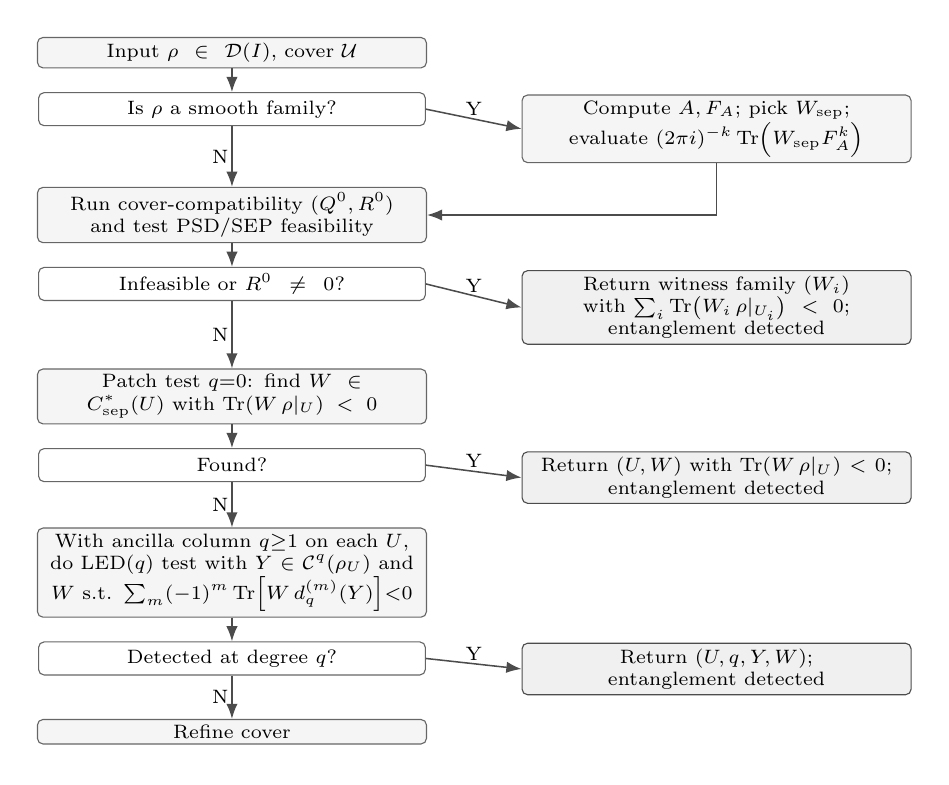
\begin{tikzpicture}[
  >=Latex,
  every node/.style={font=\scriptsize},
  RowSep/.store in=\RowSep, RowSep=3.0mm,
  ColSep/.store in=\ColSep, ColSep=12mm,
  BlockW/.store in=\BlockW, BlockW=48mm,
  block/.style  ={rectangle, rounded corners=2pt, draw=black!60, fill=gray!08,
                  align=center, inner sep=2pt, text width=\BlockW},
  dec/.style    ={rectangle, rounded corners=2pt, draw=black!60, fill=white,
                  align=center, inner sep=1.6pt, text width=\BlockW, minimum height=4.2mm},
  result/.style ={rectangle, rounded corners=2pt, draw=black!70, fill=black!6,
                  align=center, inner sep=2pt, text width=\BlockW},
  flow/.style   ={-Latex, line width=0.55pt, draw=black!70},
  lab/.style    ={font=\scriptsize, inner sep=1pt}
]
\matrix[matrix of nodes, row sep=\RowSep, column sep=\ColSep, nodes in empty cells] (M) {
  \node[block] (start) {Input $\rho\in\mathcal D(I)$, cover $\mathcal U$}; & \\
  \node[dec]   (fam)   {Is $\rho$ a smooth family?};                                      & \node[block]  (geo)    {Compute $A,F_A$; pick $W_{\rm sep}$; evaluate $(2\pi i)^{-k}\Tr(W_{\rm sep}F_A^k)$}; \\
  \node[block] (cech)  {Run cover‑compatibility $(Q^0,R^0)$ and test PSD/SEP feasibility}; & \\
  \node[dec]   (feas)  {Infeasible or $R^0\neq 0$?};                             & \node[result] (witfam) {Return witness family $(W_i)$ with $\sum_i\Tr(W_i\,\rho|_{U_i})<0$; entanglement detected}; \\
  \node[block] (qzero) {Patch test $q{=}0$: find $W\in C^*_{\rm sep}(U)$ with $\Tr(W\,\rho|_U)<0$}; & \\
  \node[dec]   (qzok)  {Found?};                                                 & \node[result] (q0out)  {Return $(U,W)$ with $\Tr(W\,\rho|_U)<0$; entanglement detected}; \\
  \node[block] (anc)   {With ancilla column $q{\ge}1$ on each $U$, do LED$(q)$ test with $Y\in\mathcal C^q(\rho_U)$ and $W$ s.t. $\sum_m(-1)^m\Tr[W\,d_q^{(m)}(Y)]{<}0$}; & \\
  \node[dec]   (anck)  {Detected at degree $q$?};                                & \node[result] (ancout) {Return $(U,q,Y,W)$; \\entanglement detected}; \\
  \node[block] (ref)   {Refine cover};                                           & \\
};

\draw[flow] (start) -- (fam);
\draw[flow] (fam.east) -- node[lab, above]{Y} (geo.west);
\draw[flow] (fam) -- node[lab, left]{N} (cech);
\draw[flow] (geo.south) |- (cech);

\draw[flow] (cech) -- (feas);
\draw[flow] (feas.east) -- node[lab, above]{Y} (witfam.west);
\draw[flow] (feas) -- node[lab, left]{N} (qzero);

\draw[flow] (qzero) -- (qzok);
\draw[flow] (qzok.east) -- node[lab, above]{Y} (q0out.west);
\draw[flow] (qzok) -- node[lab, left]{N} (anc);

\draw[flow] (anc) -- (anck);
\draw[flow] (anck.east) -- node[lab, above]{Y} (ancout.west);
\draw[flow] (anck) -- node[lab, left]{N} (ref);
\end{tikzpicture}
%\caption{Flow of the entanglement test.}
\end{figure}


\bibliographystyle{amsalpha}
\bibliography{ref}
\end{document}
